% The document class supplies options to control rendering of some standard
% features in the result.  The goal is for uniform style, so some attention 
% to detail is *vital* with all fields.  Each field (i.e., text inside the
% curly braces below, so the MEng text inside {MEng} for instance) should 
% take into account the following:
%
% - author name       should be formatted as "FirstName LastName"
%   (not "Initial LastName" for example),
% - supervisor name   should be formatted as "Title FirstName LastName"
%   (where Title is "Dr." or "Prof." for example),
% - degree programme  should be "BSc", "MEng", "MSci", "MSc" or "PhD",
% - dissertation title should be correctly capitalised (plus you can have
%   an optional sub-title if appropriate, or leave this field blank),
% - dissertation type should be formatted as one of the following:
%   * for the MEng degree programme either "enterprise" or "research" to
%     reflect the stream,
%   * for the MSc  degree programme "$X/Y/Z$" for a project deemed to be
%     X%, Y% and Z% of type I, II and III.
% - year              should be formatted as a 4-digit year of submission
%   (so 2014 rather than the academic year, say 2013/14 say).

\documentclass[ % the name of the author
                    author={Manan Vaswani},
                % the name of the supervisor
                supervisor={Dr. Raphael Clifford},
                % the degree programme
                    degree={MEng},
                % the dissertation    title (which cannot be blank)
                     title={A multi-core CPU implementation of the classical Boson Sampling algorithm},
                % the dissertation subtitle (which can    be blank)
                  subtitle={},
                % the dissertation     type
                      type={},
                % the year of submission
                      year={2019} ]{dissertation}
                      
                     
%%% Packages
\usepackage{complexity}
\usepackage{amsthm}
\usepackage{algorithm}
\usepackage[noend]{algpseudocode}
\usepackage{minted}
\usepackage{graphicx}
\usepackage{pgf}
\usepackage{capt-of}
\usepackage[export]{adjustbox}


\theoremstyle{plain}
\newtheorem{definition}{Definition}

\theoremstyle{definition}
\newtheorem{example}{Example}

\DeclareMathOperator*{\Var}{\mathrm{Var}}
\DeclareMathOperator*{\Cov}{\mathrm{Cov}}
\DeclareMathOperator*{\Per}{\mathrm{Per}}

\begin{document}

% =============================================================================

% This section simply introduces the structural guidelines.  It can clearly
% be deleted (or commented out) if you use the file as a template for your
% own dissertation: everything following it is in the correct order to use 
% as is.

% =============================================================================

% This macro creates the standard UoB title page by using information drawn
% from the document class (meaning it is vital you select the correct degree 
% title and so on).

\maketitle

% After the title page (which is a special case in that it is not numbered)
% comes the front matter or preliminaries; this macro signals the start of
% such content, meaning the pages are numbered with Roman numerals.

\frontmatter

% This macro creates the standard UoB declaration; on the printed hard-copy,
% this must be physically signed by the author in the space indicated.

\makedecl

% LaTeX automatically generates a table of contents, plus associated lists 
% of figures, tables and algorithms.  The former is a compulsory part of the
% dissertation, but if you do not require the latter they can be suppressed
% by simply commenting out the associated macro.

\tableofcontents
%\listoffigures
%\listoftables
%\listofalgorithms
%\lstlistoflistings

% The following sections are part of the front matter, but are not generated
% automatically by LaTeX; the use of \chapter* means they are not numbered.

% -----------------------------------------------------------------------------

\chapter*{Abstract}

This paper gives a study of the Boson Sampling problem and its significance to quantum supremacy, and focuses on the exact Boson Sampling Algorithm B proposed by Clifford and Clifford in 2017 \cite{clifford17}, with the objective to produce a highly optimised and efficient implementation of the algorithm. The Boson Sampling problem, introduced by Aaronson and Arkhipov in 2011 \cite{aaronson2011}, was thought to be an attainable demonstration of quantum supremacy. However, recent advances in the field of classical Boson Sampling such as a large-scale implementation of the naive algorithm by Wu et. al. in 2018 \cite{wu2018}, and more significantly, an improved algorithm for exact Boson Sampling by Clifford and Clifford which drastically reduces the theoretical runtime has reduced the likelihood of near term quantum supremacy. The implementation shown in this paper serves as stronger evidence that quantum supremacy in the field of Boson Sampling is not imminent in the near future. The implementation is run on the Blue Crystal 4 supercomputer, and achieves a speed up using a multi-threading approach. The results obtained are analysed and show promising results for the the future of classical Boson Sampling.
The implementation is available to access at: https://github.com/mananvaswani/classical-boson-sampling


% -----------------------------------------------------------------------------

\chapter*{Supporting Technologies}

\section{Blue Crystal 4} \label{sec:bc4}
I made use of the Blue Crystal Phase 4 supercomputer (henceforth abbreviated as BC4) to run most of my code. BC4 is one of the fastest and most advanced supercomputing facilities in the UK, made available by the University of Bristol High Performance Computing group \cite{blue_crystal}. Phase 4 has 525 Lenovo nx360 m5 compute nodes, each of which has two 14 core 2.4 GHz Intel E5-2680 v4 (Broadwell) CPUs, and 128 GiB of RAM. Note that such a CPU with 14 physical cores would have 28 logical cores.

\section{C\texttt{++} libraries/APIs}
\subsection{OpenMP} \label{sec:openMP}
OpenMP is an application programming interface(API) that implements multithreading, which is a method of parallelising where a master thread divides tasks among a team of threads. Concurrently, each of these threads is run individually on a single logical core. Each of the threads has an associated id, indexed starting from 0. It is possible to obtain the number of threads, or the thread index using a collection of special OpenMP functions. In C\texttt{++}, the OpenMP functions are included in a header file `omp.h'. OpenMP is used with the help of \#pragmas in C\texttt{++}, which is a compiler-specific preprocessor directive, and is used to carry out operations such as creating a team of threads or automatically dividing iterations of a loop between threads \cite{dagum1998openmp}. I used OpenMP to parallelise the algorithm in the paper. 

\subsection{Armadillo} \label{sec:armadillo}
In the implementation, I make extensive use of the C\texttt{++} Armadillo library\cite{armadillo}. Armadillo is a high quality linear algebra library that provides us with efficient implementations of matrix and vector operations. It greatly simplifies operations such as adding vectors, calculating cumulative products, and accessing matrix columns to name a few. Armadillo supports complex numbers as well, which was a necessary requirement for the project. In addition, it supports the use of OpenMP for parallelisation, and automatically uses it in some cases to speed up computationally expensive operations. Note that Armadillo stores matrices in column-order, so accessing elements column-wise may speed up operations.

\section{Intel VTune} \label{sec:vtune}
I used the Intel VTune 2018 profiler to analyse my code and identify bottlenecks. It was available to use on BC4. Code profilers like VTune dynamically analyse executable code that is running, and identify bottlenecks by giving a detailed break down of information about CPU usage, and time taken to run individual lines of the code. Intel VTune also comes with a graphical user interface which lets the user look at bottom-up approaches of performance hotspots, enabling them to easily locate time-consuming areas in the code. \cite{vtune2018}.

\section{Miscellaneous Tools}
\subsection{Python, Matplotlib}
I used the Python to process the timing data that I had obtained, and subsequently used the Matplotlib library to plot the graphs representing this data.

\subsection{Godbolt Compiler Explorer} \label{sec:godbolt}
Godbolt is an online tool that shows what high level language (such as C\texttt{++}) code ends up looking like after compilation \cite{god-bolt}. I used it to gain a deeper understanding of how some sections of my code ran.


% -----------------------------------------------------------------------------

\chapter*{Acknowledgements}

\noindent
I would like to thank my supervisor, Dr. Raphael Clifford, for his help and support throughout the year and for introducing me to the Boson Sampling problem.

% =============================================================================

% After the front matter comes a number of chapters; under each chapter,
% sections, subsections and even subsubsections are permissible.  The
% pages in this part are numbered with Arabic numerals.  Note that:
%
% - A reference point can be marked using \label{XXX}, and then later
%   referred to via \ref{XXX}; for example Chapter\ref{chap:context}.
% - The chapters are presented here in one file; this can become hard
%   to manage.  An alternative is to save the content in seprate files
%   the use \input{XXX} to import it, which acts like the #include
%   directive in C.

\mainmatter

% -----------------------------------------------------------------------------

\chapter{Contextual Background}
\label{chap:context}

\noindent
The advances made in the field of quantum algorithms in the past 25 years has given rise to questions about whether a number of classical hypotheses still hold true, in light of modern quantum research. The most notable example is the Extended Church-Turing Thesis which, in simple terms says that all computational problems that are efficiently solvable by realistic physical devices are also efficiently solvable by a probabilistic Turing machine \cite{kaye2007}. However, Shor's algorithm \cite{shor1995} potentially disproves this. Informally, Shor's discovery stated that if a classical computer could accurately simulate a quantum-mechanical experiment in probabilisitic polynomial time, then it must be able to factor integers in polynomial time as well. The problem of factoring integers is known to have no polynomial-time algorithm on a classical computer. It is so widely accepted that factoring integers is a hard problem that a number of cryptographic systems are built on its hardness, including the famous RSA algorithm \cite{rsa1978}. Hence, Shor's algorithm has a strong implication: If a classical computer is able to simulate quantum experiments efficiently, it would be able to break widely used cryptosystems such as RSA.

The topic of classically simulating quantum systems is a central idea in the field of quantum supremacy. Quantum supremacy is the phenomena that there exist quantum experiments that cannot be accurately and efficiently simulated using classical systems \cite{preskill2012}. Numerous attempts have been made to demonstrate quantum supremacy but the current physical limitations of quantum systems has made that an extremely challenging problem. Additionally, what makes quantum supremacy so hard to demonstrate is that it is not defined in terms of the ability of a quantum system to solve a particular problem, but rather it requires showing that classical computers cannot solve a problem. In a way, it could be likened to classifying computational problems into complexity classes \cite{papadimitriou2003}. In the same way that a number of complexity theory related theorems and conjectures rely on a number of theoretic assumptions, it is necessary for quantum supremacy to rely on similar such assumptions as well, as it would be nearly impossible to unconditionally prove such statements \cite{harrow2017}. Linking back to Shor's algorithm and its potential to demonstrate quantum supremacy and simultaneously disprove the Extended-Church Turing thesis, there are two significant drawbacks which prevent it from doing so. 

Firstly, the problem of factoring integers, while widely believed to be an $\NP-\text{hard}$ problem, its hardness has not been formally proved. The assumption is not strong enough to verify that Shor's algorithm does indeed achieve quantum supremacy.

The second, and more obvious drawback to Shor's algorithm is that a large-scale physical implementation of a quantum computer to run it is beyond the current reach of technology. While there have been several experiments that successfully factor small numbers like 15 \cite{monz2016} and 21 \cite{vartiainen2004} with high accuracy, we are not at risk of RSA breaking just yet!

This has motivated the search for other such quantum experiments that can be run physically, but not simulated classically. However, an important requirement is that it should be possible to model these experiments as computational problems in order to study their hardness.

There are a handful of problems that satisfy this criteria, such as the problem of sampling the output distribution of random quantum circuits, which has been one of the most popular problems in the field of quantum supremacy in the past few years due to a lot of interest from big companies like Google and IBM. The best known classical algorithm for simulating the task of sampling bitstrings from the output of random quantum circuits is exponential in the number of qubits in the bitstring, leading one group of researchers in 2016 to estimate that a physical experiment with $\approx 50$ qubits could be enough to demonstrate quantum supremacy \cite{boixo2016}. However, more recently a classical simulation of the problem with 56 qubits was carried out successfully \cite{pednault2017}. This pushed the imminence of quantum supremacy for the circuit sampling problem even further away.

The other famous problem in the field of quantum supremacy, of a similar flavour, is the Boson Sampling problem, which is the main focus of this paper. While the problem reduces down to a sampling problem like circuit sampling, as the name suggests, it actually belongs to a paradigm of Quantum Computation different to the ones discussed before, called Linear Optical Quantum Computation (or LOQC). The protocol by Knill, Laflamme and Milburn in 2001 \cite{knill2001} demonstrated that a scalable quantum computer with linear optical elements could be robustly implemented. In LOQC, a photon is used to represent a single qubit.

Aaronson and Arkhipov in their paper on the classical complexity of linear optics showed that it was possible to build a quantum computation model within the LOQC paradigm which could not be efficiently simulated by classical computers \cite{aaronson2011}. They define a model for `Boson Sampling' in which $n$ identical photons are passed through a linear optical network and then measured to determine their location. This linear optical network consists of a collection of simple optical elements called beam splitters and phase shifters.

\begin{figure}
	\centering
  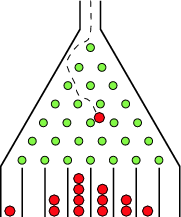
\includegraphics[width=15em]{galton_board}
  \caption{A Galton board, used to demonstrate sampling from a binomial distribution \cite{galton_board}}
  \label{fig:galton_board}
\end{figure}

The model could be thought of as being a parallel to a Galtons Board, shown in figure \ref{fig:galton_board}, in which $n$ balls are dropped into a vertical lattice of wooden pegs, each of which randomly scatters an incoming ball to one of two other pegs with equal probability. The input to this system is the exact arrangement of the pegs, while the output is the number of balls that have landed at each location on the bottom. The output could alternatively be thought of as a sample from the distribution of all possible output arrangements (which is the binomial distribution in this case).

In the Aaronson and Arkhipov Boson Sampling model, the balls are replaced with identical photons, and the pegs arranged in a lattice are replaced with an arbitrary arrangement of optical elements. Also, the photons can be dropped from different starting locations as opposed to just a single position. The Boson-Sampling problem involves sampling the output distribution using photon-number discriminating detectors. They argued that if there is a polynomial time classical algorithm that exactly samples from the Boson Sampling distribution, the complexity class $\P^{\#\P} = \BPP^{\NP} $  which would collapse the polynomial hierarchy to the third level by Toda's theorem \cite{toda1991}.

In order to actually compare the physical model with a classical computational model, the paper reduces the Boson Sampling problem to a problem in purely mathematical terms. Photons are a type of boson, which is one of the two main types of particles in the world. The link between bosons and permanents of matrices has been known since 1953, from the work by Caianiello \cite{Caianiello1953} which showed that the amplitudes of $n$-boson process can be written as the permanents of $n \times n$ matrices. Hence it was possible to represent the Boson Sampling distribution in terms of the permanents of matrices, and this was shown and proved in the paper.

Carrying out a physical experiment for Boson Sampling is not a trivial task, and increasing the number of photons or the number of output modes to large enough values is extremely difficult. The current experimental record is with 5 photons and 9 output modes. However, this does show the possibility of potentially having larger-scale implementations in the future.

The Aaronson and Arkhipov paper provoked much interest in the study of classical computation algorithms for Boson Sampling. Much of the work is focused around fast implementations for the calculation of permanents of large matrices, with recent works showing efficient results for matrices as large as $54 \times 54$ \cite{roga2019, lundow2019}. There have been a few other approaches to simulating the Boson sampling problem such as classically modelling the linear optical network itself, and sampling from the output as opposed to computing the purely mathematical equivalent of the problem \cite{rahimi2016}. There have also been attempts at using Markov Chain Monte Carlo (MCMC) methods to sample from the Boson Sampling distribution by trying to identify it as the equilibrium distribution of a Markov chain, following the method by Hastings \cite{hastings1970}. However, estimating how accurately these methods approximate to the true Boson Sampling experiment has been difficult. Nonetheless, the MCMC method proposed by Neville et. al. \cite{neville2017} gave strong numerical evidence that classical Boson Sampling may be feasible for large input sizes.

In terms of actual implementations of the Boson Sampling algorithm, there have been few, with the most significant benchmark being the test of the simulation run on the Tianhe-2 supercomputer \cite{wu2018} which managed to simulate Boson Sampling for 50 photons with a runtime of approximately 100 minutes.

However, in the groundbreaking paper by Clifford and Clifford \cite{clifford17}, a new significantly faster algorithm was proposed which showed promise of carrying out classical Boson Sampling in an even shorter time. The algorithm proposed in this paper is central to our work. We give a highly optimised implementation of this algorithm with the aim of setting a new benchmark for the classical Boson Sampling problem, and in the process pushing away the imminence of quantum supremacy in the near future.
\\
\\
\noindent
Building on the content discussed in this section, the concrete aims of the project are:
\begin{enumerate}
\item Research and analyse literature on the Boson Sampling problem, and its relation to quantum supremacy.
\item Demonstrate a strong understanding of the Boson Sampling problem, and the algorithms proposed in \cite{clifford17}.
\item Study potential techniques to optimise an implementation of the algorithm, and provide a high-speed CPU implementation of the algorithm.
\item Summarise the results obtained by optimising the implementation, and state its implications.
\end{enumerate}

% -----------------------------------------------------------------------------

\chapter{The Boson Sampling Algorithm}
\label{chap:bosonSampling}

\section{Mathematical Preliminaries}
Before we can explain the problem in a mathematical sense and go on to state the algorithms used to solve it, it is essential to understand a few mathematical concepts.
\subsection{Binary Gray Code} \label{sec:gray_code}
The Gray code, or Reflected Binary Code is a special ordering of numbers in binary where two consecutive numbers have exactly one bit changed \cite{Nijenhuis1978}. The Gray code for the first 15 numbers is shown in table \ref{tab:gray_code_prelim}.

\begin{table}[h!]
  \begin{center}
    \caption{Elements of Gray code from 0 to 15}
    \label{tab:gray_code_prelim}
    \begin{tabular}{|c|c c c c|| c| c c c c|}
    \hline
      \textbf{Decimal} & \multicolumn{4}{|c||}{\textbf{Gray code}} & \textbf{Decimal} & \multicolumn{4}{|c|}{\textbf{Gray code}}\\
      \hline
      0 & 0 & 0 & 0 & 0 & 8 & 1 & 1 & 0 & 0\\
      1 & 0 & 0 & 0 & 1 & 9 & 1 & 1 & 0 & 1\\
      2 & 0 & 0 & 1 & 1 & 10 & 1 & 1 & 1 & 1\\
      3 & 0 & 0 & 1 & 0 & 11 & 1 & 1 & 1 & 0\\
      4 & 0 & 1 & 1 & 0 & 12 & 1 & 0 & 1 & 0\\
      5 & 0 & 1 & 1 & 1 & 13 & 1 & 0 & 1 & 1\\
      6 & 0 & 1 & 0 & 1 & 14 & 1 & 0 & 0 & 1\\
      7 & 0 & 1 & 0 & 0 & 15 & 1 & 0 & 0 & 0\\
      \hline
    \end{tabular}
  \end{center}
\end{table}

\subsection{Permanent of a matrix} \label{sec:permanent}
Computing the permanent of large matrices is one of the key parts of the Boson Sampling problem, as will be discussed in detail while explaining the problem in the subsequent sections of the paper.
\begin{definition}{\cite{marcus_minc66}}
The permanent of an $n \times n$ matrix $A = (a_{ij})$ is defined as
\begin{equation}
\Per A = \sum_{\sigma \in S_n} \prod_{i=1}^n a_{i\sigma(i)}
\end{equation}
where the sum is over all elements of the symmetric group $S_n$ i.e. over all permutations of the numbers in $[n] = \{1, 2, ... , n\}$.
\end{definition}

\begin{example}
For a $2 \times 2$ matrix, the permanent is calculated as follows
\begin{equation}
\Per 
\begin{bmatrix}
a & b \\
c & d
\end{bmatrix}
= ad + bc
\end{equation}
\end{example}
\begin{example}
For a $3 \times 3$ matrix, the permanent is calculated as follows
\begin{equation}
\Per 
\begin{bmatrix}
a & b & c\\
d & e & f\\
g & h & i\\ 
\end{bmatrix}
= aei +bfg + cdh + ceg + bdi + afh
\end{equation}
\end{example}
One can observe that the definition of the permanent is similar to the more commonly used determinant function, differing in the fact that the permanent definition lacks the alternating signs. An important property to note about the permanent function is that it is invariant to transposition i.e. $\Per A = \Per A^T$ \cite{ryser_1963}.

\subsubsection{Computing the permanent}\label{prelim_permanent_calc}
Valiant showed that the problem of computing the permanent of a matrix is in the class $\# \P$-complete which implies that it is unlikely to have a polynomial time algorithm \cite{valiant1979}. The naive algorithm obtained by directly translating the formula into an algorithm would run in $\mathcal{O}(n!n)$ time.

A significant improvement on the naive approach, Rysers algorithm uses a variant of the inclusion-exclusion principle and can be evaluated in $\mathcal{O}(n^2 2^n)$ time  \cite{ryser_1963}. Nijenhuis and Wilf sped this up to $\mathcal{O}(n2^n)$ time by iterating over the sum in Gray code order \cite{Nijenhuis1978}.

Another formula that is as fast as Rysers was independently derived by Balasubramanian\cite{balasubramanian1980}, Bax\cite{bax1998}, Franklin and Bax\cite{bax1996}, and Glynn\cite{glynn2010}, all using different methods. This shall henceforth be referred to as Glynn's formula and it is described as follows.

Let $M = (m_{ij})$ be an $n \times n$ matrix with $m_{ij} \in \mathbb{C}$, then
\begin{equation}
\Per M = \frac{1}{2^{n-1}} \sum_\delta \left( \prod_{k=1}^n \delta_k \right) \prod_{j=1}^n\sum_{i=1}^n \delta_i m_{ij}
\end{equation}
where $\delta \in \{-1, 1\}^n$ with $\delta_1 = 1$. Hence there are $2^{n-1}$ such values for $\delta$.

Implementing the formula as is would require $\mathcal{O}(2^n n^2)$ time. However, iterating over the $\delta$ arrays in Gray code order reduces it to $\mathcal{O}(n 2^n)$ time.

In order to exploit this trick, let $v_j$ be the symbol used to denote the innermost sum i.e. $v_j = \sum_{i=1}^n \delta_i m_{ij}$. If $\delta$ is iterated over in Gray code order, then one can notice that the terms $\{ v_j, j \in [n]\}$ can actually be computed in $\mathcal{O}(n)$ time for a given value of $\delta$ rather than $\mathcal{O}(n^2)$ which is how long it would take if done naively. This is because successive elements of $\delta$ differ in only one position, so each successive $v_j$ differs only by the addition or subtraction of some $m_{ij}$ where $i$ is the position at which $\delta$ was last changed. Hence, the product of $v_j$ terms can now be calculated in $\mathcal{O}(n)$ time. Note that $\delta \in \{-1, 1\}^n$ but elements of the Gray code of size $n$ are in $\{0, 1\}^n$. To resolve this, map each 0 in the Gray code to a 1 of the $\delta$ array, and each 1 in the Gray code to a -1 of the $\delta$ array.

\subsection{Specifying the problem}
A summary of the problem in purely mathematical terms, as explained in \cite{clifford17} and \cite{aaronson2011} is as follows.

Let $m$ and $n$ be positive integers. Consider all possible multisets\footnote{A multiset is a special kind of set in which elements can be repeated} of size $n$ with elements in $[m]$, where $[m] = \{1, ... , m\}$. Let $\mathbf{z} = [z_1, z_2, ... , z_n]$ be an array representation of such a multiset, with its elements in non-decreasing order. In other words, $\mathbf{z}$ is an array of $n$ integers taken from $[m]$ (with repetition) and arranged in non-decreasing order. Define $\Phi_{m,n}$ to be the set of all distinct values that $\mathbf{z}$ can take. Define $\mu(\mathbf{z}) = \prod_{j=1}^m s_j !$ where $s_j$ is the multiplicity of $j$ in the array $\mathbf{z}$ i.e. the number of times it appears in $\mathbf{z}$.

$A = (a_{ij})$ is a complex-valued $m \times n$ matrix constructed by taking the first $n$ columns of a given $m \times m$ Haar random unitary matrix. For each $z$, build an $n \times n$ matrix $A_\mathbf{z}$ where the $k^{\text{th}}$ row of $A_\mathbf{z}$ is the $z_k^{\text{th}}$ row in $A$, for $k = 1, ... , n$. Finally, define a probability mass function over $\Phi_{m,n}$  as
\begin{equation}\label{boson_sampling_formula1}
q (\mathbf{z}) = \frac{1}{\mu(z)} \left|\Per A_\mathbf{z} \right| ^2 = \frac{1}{\mu(\mathbf{z})}  \left|\sum_{\sigma} \prod_{k=1}^n a_{z_k \sigma_k}\right|^2, \quad \mathbf{z} \in \Phi_{m,n}
\end{equation}
where $\Per A_\mathbf{z}$ is the permanent of $A_\mathbf{z}$ and $\pi[n]$ is the set of all permutations of $[n]$.

The computing task is to simulate random samples from the above pmf $q(z)$. This mathematical definition was shown to be equivalent to the physical experiment by Aaronson and Arkhipov \cite{aaronson2011}.
\subsubsection{Calculating the size of the sample space}
The size of the sample space $ \Phi_{m,n}$ can be calculated using the `stars and bars' technique from combinatorics \cite{feller1968}. In our problem, we have $n$ `stars' representing arbitrary elements of the array $z$, and $m$ `buckets' representing all the values in $[m]$. Recall that $z$ is a sorted array representation of a multiset, so multiple `stars' can be in one `bucket'. Since there are $m$ `buckets', we need $m-1$ `bars' to divide the `stars' into `buckets'. Therefore, from a total of $m-1 + n$ objects, we need to pick $n$ of these to be the `stars'. There are $\binom{m+n-1}{n}$ ways to do this. Hence, there are $\binom{m+n-1}{n}$ possible values of $z$.

\section{The naive algorithm}
Translating the formula above (Equation \ref{boson_sampling_formula1}) directly to an algorithm would require $\mathcal{O}(\binom{m+n-1}{n} n 2^n)$ time to evaluate. The $\binom{m+n-1}{n}$ term comes from the size of the sample space of the pmf, and calculating the value of the permanent using the fastest known methods takes $\mathcal{O}(n 2^n)$ time (Section \ref{prelim_permanent_calc}). With $m = \mathcal{O}(n^2)$ as suggested in \cite{aaronson2011}, the total running time is $\mathcal{O}(\binom{n^2+n-1}{n} n 2^n)$. Hence, even for values of $n$ as small as 5 or 6, computing the Boson Sampling problem would be intractable for even very powerful supercomputers.

\begin{algorithm}
\caption{Boson Sampler (Naive Algorithm): Single sample $\mathbf{z}$ from $q(\mathbf{z})$ in $\mathcal{O}(\binom{m+n-1}{n} n 2^n)$ time}
\begin{algorithmic}[1] \label{alg:naive}
\Require $m, n \in \mathbb{Z}_+$; $A$ formed by first $n$ columns of $m \times m$ Haar random unitary matrix
\State $w_i \leftarrow \frac{1}{\mu(\mathbf{x})} \left| \Per A_\mathbf{x} \right| ^2, \mathbf{x} \in \Phi_{m,n}$ \Comment{Make indexed weight array $\mathbf{w}$}
\State $\mathbf{z} \leftarrow \text{Sample}(w)$  \Comment{Sample array $\mathbf{z}$ from $\mathbf{w}$}
\State \textbf{return} $\mathbf{z}$
\end{algorithmic}
\end{algorithm}

In the literature \cite{clifford17}, two new algorithms are proposed for exact Boson Sampling. These are referred to as Algorithm A and Algorithm B, and both provide a significant speed up on the naive algorithm. The following subsections summarise the approach taken to obtain them.

\section{Algorithm A}
The approach to Algorithm A starts by expanding the sample space to a much larger size, which seems counterintuitive at first, but it allows us to express the pmf (Equation \ref{boson_sampling_formula1}) in a form that is much easier to compute. The sample space is expanded to the space of all arrays $\mathbf{r}=(r_1, r_2, ... , r_n)$ where each element $r_k$ is in $[m]$, which implies that we are considering a distribution on the product space $[m]^n$. It is stated and proved that sampling from $q(\mathbf{z})$ is equivalent to sampling from the pmf
\begin{equation} \label{eqn:algADistribution}
p(\mathbf{r}) = \frac{1}{n!} \left| \Per A_\mathbf{r} \right| ^2 = \frac{1}{n!} \left| \sum_\sigma \prod_{i=1}^n a_{r_i \sigma_i} \right| ^2 , \quad \mathbf{r} \in [m]^n 
\end{equation}
where as before, $\sigma$ is the set of all permutations of $[n]$.

This method requires $p(\mathbf{r}) = p(r_1, ... , r_n)$ to be rewritten as a product of conditional probabilities using the chain rule i.e.
\begin{equation}\label{eqn:bosonSamplingConditional}
p(\mathbf{r}) = p(r_1)p(r_2 | r_1) p (r_3 | r_1, r_2) ... p(r_n | r_1, r_2, ... , r_{n-1})
\end{equation}

We first sample $r_1$ from $p(r_1), r_1 \in [m]$. Then for $k=2, .. n$, we sample $r_k$ from the conditional pmf $p(r_k | r_1, r_2, ... , r_{k-1})$ with $r_1, ... , r_{k-1}$ fixed. After sampling all values of $r_k$, sort $(r_1, r_2, ... , r_n)$ in non-decreasing order, and that results in the array representation of a multiset sampled from the Boson Sampling distribution $q(\mathbf{z})$. In order to calculate the conditional probabilities, a formula for the joint pmf of the leading subsequences of $(r_1, ... , r_k)$ is given in Lemma 1 of the paper, and proved using arithmetic techniques and facts about probability measures. The formula in Lemma 1 is as follows:
\begin{equation} \label{eq:lemma1}
p(r_1, ... , r_k) = \frac{(n-k)!}{n!} \sum_{c \in \mathcal{C}_k} \left| \Per A_{r_1, ... , r_k}^c \right| ^2 , \quad k = 1, ... , n
\end{equation}
where $\mathcal{C}_k$ is the set of $k-$combinations taken without replacement from $[n]$ and $A_{r_1, ... , r_k}^c$ is the matrix formed by taking only columns $c \in \mathcal{C}_k$ of the rows $(r_1, ... , r_k)$ of $A$.

Notice in equation \ref{eqn:bosonSamplingConditional}, we need to sample $r_k$ from the conditional probability distribution $p(r_k | r_1, ... , r_{k-1})$. This can be rewritten as $p(r_1, ... , r_k)/p(r_1 ... r_{k-1})$. Since $r_k$ does not appear in the denominator, in order to sample $r_k$ from the conditional pmf, we can equivalently sample from the pmf proportional to the numerator, as $(r_1, ... r_{k-1})$ are fixed, known values at this stage in the algorithm. Therefore, the formula is Lemma 1 (Formula \ref{eq:lemma1}) is used to calculate the conditional pmfs at each stage, giving way to Algorithm B.

\begin{algorithm}
\caption{Boson Sampler (Algorithm A): Single sample $\mathbf{z}$ from $q(\mathbf{z})$ in $\mathcal{O}(mn3^n)$ time}
\begin{algorithmic}[1]
\Require $m, n \in \mathbb{Z}_+$; $A$ formed by first $n$ columns of $m \times m$ Haar random unitary matrix
\State $\mathbf{r} \leftarrow 0 $ \Comment{Empty array}
\For{{$k \leftarrow 1 \text{ to } n$}
\State $w_i \leftarrow \sum_{c \in \mathcal{C}_k} \left| \Per A_{(\mathbf{r}, i)}^c \right| ^2, i \in [m] $ \Comment{Make indexed weight array $\mathbf{w}$}
\State $x \leftarrow \text{Sample}(w)$ \Comment{Sample index $x$ from $\mathbf{w}$}
\State $\mathbf{r} \leftarrow (\mathbf{r}, x)$} \Comment{Append $x$ to $\mathbf{r}$}
\EndFor
\State $\mathbf{z} \leftarrow \text{IncSort}(\mathbf{r})$ \Comment{Sort $\mathbf{r}$ in non-decreasing order}
\State \textbf{return} $\mathbf{z}$
\end{algorithmic}
\end{algorithm}

The correctness of the algorithm is clear as it is simply an evaluation of the required pmf using the chain rule of probability. The literature gives a mathematical proof to derive the runtime, however here we shall give an informal explanation to obtain the runtime using the algorithm above. The runtime is dominated by the loop in lines 2 to 6, as the sorting step in line 7 takes only $\mathcal{O}(n \log n)$ using the fastest methods for sorting such as quicksort. In each iteration of the for loop, we first construct the conditional pmf on the sample space $[m]$. This is represented by a weighted array $\mathbf{w}$ and requires calculating the permanents of $\left|\mathcal{C}_k\right|$ $k \times k$ matrices for each $i \in [m]$, where $k$ is the loop index variable. Sampling from this distribution (line 4) takes $\mathcal{O}(m)$ time \cite{walker1974}, but this too is dominated by the calculations in line 3, so we can ignore it. Therefore, the total time taken in the $k^\text{th}$ iteration is $\mathcal{O}(m \binom{n}{k} k 2^k)$, as $\left|\mathcal{C}_k\right| = \binom{n}{k}$ and calculating the permanent of a $k \times k$ matrix takes $\mathcal{O}(k 2^k)$ using the fastest methods (Section \ref{prelim_permanent_calc}). So for $n$ iterations,
\begin{equation}
\sum_{k=1}^n m k 2^k \binom{n}{k} = m \frac{2}{3} n 3^n = \mathcal{O}(mn3^n)
\end{equation}
Therefore the total time taken is $\mathcal{O}(mn3^n)$. In terms of space complexity, we only need to store one permanent calculation at a time, and the weight array for each pmf is of size $m$. These can also be stored only one at a time, so $\mathcal{O}(m)$ additional space is required.


\section{Algorithm B} \label{sec:algB}
The main theorem of the paper \cite{clifford17} (Theorem 1) states that the time complexity of the Boson Sampling problem is $\mathcal{O}(n2^n + \text{poly}(m, n))$ where $ \text{poly}(m, n) = \mathcal{O}(mn^2)$, with $\mathcal{O}(m)$ additional space required. This is achieved using the second algorithm proposed in the paper i.e. Algorithm B.

Algorithm B makes use of the Laplace Expansion \cite{marcus_minc66} of permanents to obtain a significant speed up. The Laplace expansion allows us to calculate the permanent of a matrix using its permanent minors (the permanent of a submatrix with a column and a row removed). For any $k \times k$ matrix $B = (b_{i,j})$,
\begin{equation}
\Per B = \sum_{l=1}^k b_{k, l} \Per B_{k, l}^{\diamond},
\end{equation}
where $B_{k, l}^{\diamond}$  is the submatrix of $B$ with row $k$ and column $l$ removed. Hence the permanent of $B$ can be calculated in $\mathcal{O}(k)$ steps provided the permanent minors i.e. the values $\{ \Per B_{k, l}^{\diamond} \}$ are known.

Computing $\{ \Per B_{k, l}^{\diamond} \}$ by calculating each of the permanents independently would collectively take $\mathcal{O}(k^2 2^k)$ time as there are $k$ permanents to compute and to compute the value of each one takes $\mathcal{O}(k 2^k)$ time. Lemma 2 of the paper states that the collection $\{ \Per B_{k, l}^{\diamond} \}$ can be collectively evaluated in $\mathcal{O}(k 2^k)$ time and $\mathcal{O}(k)$ extra space. Using Glynn's formula to evaluate a permanent minor for a given value of $l$, we have
\begin{equation}
\Per B_{k, l}^{\diamond} = \frac{1}{2^{k-2}} \sum_\delta \left( \prod_{i=1}^{k-1} \delta_i \right) \prod_{j \in [k] \setminus l} v_j (\delta), \quad l \in [k],
\end{equation}
where $\delta \in \{-1, 1\}^{k-1}$ with $\delta_1 = 1$ and $v_j (\delta) = \sum_{i=1}^{k-1} \delta_i b_{ij}$.
The usual trick of iterating over the values of $\delta$ in Gray code order is required to compute $\Per B_{k, l}^{\diamond}$ in $\mathcal{O}(k2^k)$ time for each value of $l$, but this would still have to be repeated $k$ times to cover all $l \in [k]$. The second and more novel trick used to achieve an additional speed up is used while calculating the products $\prod_{j \in [k] \setminus l} v_j (\delta)$. Observe that for each $l$, $\prod_{j \in [k] \setminus l} v_j (\delta) = \prod_{j \in [k]} v_j (\delta) / v_l(\delta)$. However, we cannot use this method to compute the partial product as it would not work for cases when $v_l(\delta) = 0$. Instead, we first precompute two arrays $\mathbf{f}$ and $\mathbf{b}$ containing the forwards and backwards cumulative products of $\mathbf{v}(\delta) = \{v_j(\delta), j\in [k]\}$ respectively as follows,
\begin{equation}
f_i = \prod_{j=1}^i v_j(\delta), \quad f_0 = 1,
\quad b_i = \prod_{j=i}^k v_j(\delta), \quad b_{k+1} = 1 \quad i \in [k].
\end{equation}
Then each partial product $\prod_{j \in [k] \setminus l} v_j (\delta)$ can be expressed as a product of two terms from $\mathbf{f}$ and $\mathbf{b}$, $f_{l-1} b_{l+1}$ for any $l \in [k]$. Since it takes $\mathcal{O}(k)$ time to compute the forward and backward cumulative product arrays (which is done only once per $\delta$) and $\mathcal{O}(1)$ time to obtain each partial product $\prod_{j \in [k] \setminus l} v_j (\delta)$, for each value of $\delta$, the total time taken to simultaneously calculate the values of $\{ \Per B_{k, l}^{\diamond} \}$ is $\mathcal{O}(k2^k)$. Additional space required to store the partial products is $\mathcal{O}(k)$.

Coming back to formulating the second Boson Sampling algorithm, the sample space is now expanded even further with an auxiliary array $\mathbf{\alpha} = (\alpha_1, \alpha_2, ... , \alpha_n)$ where $\mathbf{\alpha} \in \pi(n)$, which is the set of permutation of $[n]$. The approach is similar to that of Algorithm A in that the goal is to create a succession of pmfs for leading subsequences of $\mathbf{r}$ and then progressively sample $r_i$ from conditional pmfs on $(r_1, ... , r_{i-1})$. The conditioning variable $\mathbf{\alpha}$ helps us reformulate the pmf in such a way that we can use the permanent minors which we are able to calculate efficiently, while still ensuring that it is equivalent to sampling from the pmf $p(\mathbf{r})$ in Equation \ref{eqn:algADistribution}.
Define
\begin{equation}
\phi(r_1, ... r_k | \mathbf{\alpha}) = \frac{1}{k!} \left| \Per A_{r_1, ... r_k}^{[n] \setminus \{\alpha_{k+1},  ... , \alpha_n\}} \right|^2, \quad k = 1, ... , n-1.
\end{equation}
In Lemma 3 of the paper, it is shown that $p(\mathbf{r}) = \mathbb{E}_{\mathbf{\alpha}}\{\phi(\mathbf{r} | \mathbf{\alpha})\}$, which is the expectation taken over $\mathbf{\alpha}$, uniformly distributed over $\pi(n)$ for fixed $\mathbf{r}$. The chain rule of expectation is used to prove the equality, and this full proof is provided in the literature. As with Algorithm A, a chain of conditional pmfs as follows is used,
\begin{equation} \label{eqn:algBChainRule}
\phi(\mathbf{r} | \mathbf{\alpha}) = \phi(r_1 | \mathbf{\alpha}) \phi(r_2 | r_1, \mathbf{\alpha}) \phi(r_3 | r_1, r_2, \mathbf{\alpha}) ... \phi(r_n | r_1, ... r_{n-1}, \mathbf{\alpha}), 
\end{equation}
where $\phi(r_k | r_1, ... r_{k-1}, \mathbf{\alpha}) = \phi(r_1, r_2, ... r_k | \mathbf{\alpha}) / \sum_{r_k} \phi(r_1, ... r_k | \mathbf{\alpha})$ using conditional probabilities and the law of total probability. The algorithm starts off by sampling $r_1$ from the pmf $\phi(r_1 | \mathbf{\alpha})$. Then for stages $k = 2 , ... , n$, $r_k$ is sampled from $\phi(r_k | r_1, ... r_{k-1}, \mathbf{\alpha})$ with $(r_1, ... , r_{k-1})$ fixed. Since the terms in the denominator are fixed, known values, sampling from $\phi(r_k | r_1, ... r_{k-1})$ is equivalent to sampling from the numerator, which can be evaluated by taking advantage of the Laplace Expansion of permanents. At stage $n$, the array $(r_1, ... , r_n)$ will have been sampled from $p(\mathbf{r})$. Sorting $(r_1, ... , r_n)$ in non-decreasing order gives $\mathbf{z}$, the array representation of the multiset sampled from the Boson Sampling distribution $q(\mathbf{z})$.
\begin{algorithm}
\caption{Boson Sampler (Algorithm B): Single sample $\mathbf{z}$ from $q(\mathbf{z})$ in $\mathcal{O}(n2^n + \text{poly}(m, n))$ time}
\begin{algorithmic}[1]
\Require $m, n \in \mathbb{Z}_+$; $A$ formed by first $n$ columns of $m \times m$ Haar random unitary matrix
\State $\mathbf{r} \leftarrow \O $	\Comment{Empty array}
\State $A \leftarrow \text{Permute}(A)$	\Comment{Randomly permute columns of $A$}
\State $w_i \leftarrow \left|a_{i, 1}\right|^2, i \in [m]$	\Comment{Make indexed weight array $\mathbf{w}$}
\State $x \leftarrow \text{Sample}(w)$	\Comment{Sample index $x$ from $\mathbf{w}$}
\State $\mathbf{r} \leftarrow (\mathbf{r}, x)$	\Comment{Append $x$ to $\mathbf{r}$}
\For{$k \leftarrow 2 \text{ to } n$}
\State $B_k^\diamond \leftarrow A_{\mathbf{r}}^{[k]}$
\State Compute  $\{ \Per B_{k, l}^{\diamond}, l \in [k] \}$	\Comment{From Lemma 2}
\State $w_i \leftarrow \left| \sum_{l = 1}^k \Per B_{k, l}^{\diamond} \right| ^2, i \in [m] $	\Comment{Using Laplace Expansion}
\State $x \leftarrow \text{Sample}(w)$
\State $\mathbf{r} \leftarrow (\mathbf{r}, x)$
\EndFor
\State $\mathbf{z} \leftarrow \text{IncSort}(\mathbf{r})$	\Comment{Sort $\mathbf{r}$ in non-decreasing order}
\State \textbf{return} $\mathbf{z}$
\end{algorithmic}
\end{algorithm}

Correctness holds as Algorithm B samples from successive conditional pmfs, which is equivalent to sampling from $\phi (r | \mathbf{\alpha})$ due to the chain rule of probability (Equation \ref{eqn:algBChainRule}), for a given $\mathbf{\alpha}$. Since  $\mathbf{\alpha}$ is uniformly distributed over the sample space $\pi(n)$, the algorithm equivalently samples from $\mathbb{E}_{\mathbf{\alpha}}\{\phi(\mathbf{r} | \mathbf{\alpha})\}$ which is shown to be equal to $p(r)$ in Lemma 3.

Once again, we will analyse the time complexity of the algorithm by going through the actual steps of the algorithm rather than the more mathematical explanation given in \cite{clifford17}. The time complexity of the algorithm is dominated by the loop as expected. Permuting the columns of $A$ (Line 2) can be carried out in $\mathcal{O}(n)$ time using the Knuth shuffling algorithm \cite{knuth1969}. Lines 3 and 4 take $\mathcal{O}(m)$ time, in order to generate the weight array representing the pmf and sample from it. In the loop from lines 6 to 11, computing the permanent minors (Line 8) takes $\mathcal{O}(k 2^k)$ time in the $k^{\text{th}}$ iteration, as discussed previously. Subsequently, the weight array in Line 9 is computed in $\mathcal{O}(mk)$ time as it is an array of size $m$, with each element taking $\mathcal{O}(k)$ time to compute as it is a sum of $k$ known terms. Sampling from this pmf (Line 10) takes $\mathcal{O}(m)$ time. The final sorting step outside the loop, in Line 12 takes $\mathcal{O}(n \log n)$ time, so it is dominated by the loop. Each iteration of the loop takes $\mathcal{O}(k 2^k) + \mathcal{O}(mk)$ time in total. So for all iterations, this takes
\begin{equation}
\sum_{k=2}^n \mathcal{O}(k2^k) + \mathcal{O}(mk) = \mathcal{O}(n2^n) + \mathcal{O}(mn^2)
\end{equation}
time. The space is dominated by the weight array in Line 9, which is of size $\mathcal{O}(m)$.

Hence, the Boson Sampling Problem can be run in $\mathcal{O}(n2^n + \text{poly}(m, n))$ time using Algorithm B.

% -----------------------------------------------------------------------------

\chapter{Algorithm Implementation}
\label{chap:execution}

In this chapter, we will discuss the actual implementation of Algorithm B described in Section \ref{sec:algB}. The paper by Clifford and Clifford which demonstrated the two new algorithms is still relatively new, which explains why there are not been any open-source large scale benchmark tests for implementations of the algorithm.

\section{Original R Implementation} \label{sec:r_code}
At the time of writing this paper, the only open-source implementation is at \cite{clifford_r2017}, by the authors of the paper. The implementation is in written as a package written in R and is freely available to download and use from CRAN \cite{cran}. This package, named `Boson Sampling' contains an implementation of Algorithm B, along with the required functions that it depends on. The relevant functions from the package are described below.
\begin{description}
\item[\mintinline{R}{bosonSampler}] \hfill \\ The package provides a function \mintinline{R}{bosonSampler(A, sampleSize, perm=FALSE)}, which implements the Boson Sampling Algorithm B from \cite{clifford17}. As the function definition suggests, it takes three arguments:
\begin{itemize}
\item \mintinline{R}{A}: The first $n$ columns of an $m \times m$ random unitary matrix.
\item \mintinline{R}{sampleSize}: The number of independent sample values to be taken from the distribution, where each value is a vector of size $n$.
\item \mintinline{R}{perm}: Takes the value \mintinline{R}{TRUE} if the permanents and pmfs associated to each sample are required to be returned. By default, \mintinline{R}{perm=FALSE} unless specified otherwise.
\end{itemize}
Note that we do not need to explicitly provide the values $m$ and $n$ as the algorithm suggests since those values are obtained by simply checking the dimensions of the input $m \times n$ matrix using the \mintinline{R}{ncol(A)} and \mintinline{R}{nrow(A)} functions from R. This implementation allows us to obtain multiple samples from the Boson Sampling distribution using the same input matrix $A$ by repeatedly looping over the algorithm the desired number of times. One notable difference is that the input matrix $A$ is transposed right at the start, with the reason being that R stores matrices in column order so transposing the matrix makes operations quicker. When accessing elements of $A$, the indices have been adjusted accordingly. Semantically, the function implements the algorithm exactly as it is, which ensures its' correctness (provided the inputs received and additional functions used are also correct).
\item[\mintinline{R}{cxPermMinors}] \hfill \\ The package provides a set of functions for computing permanents of matrices: \mintinline{R}{cxPerm(A)}, \mintinline{R}{rePerm(B)}, \mintinline{R}{cxPermMinors(C)}. Algorithm B requires the values $\{ \Per B_{k, l}^{\diamond}, l \in [k] \}$ to be computed in each iteration of the loop, and in order to do this, the \mintinline{R}{bosonSampler} function makes a call to the \mintinline{R}{cxPermMinors} function. This function takes an input matrix $A$ of size $k \times k-1$. Note that this is actually the transpose of the $B_k^{\diamond}$ in Line 7 of the algorithm, since the original matrix in \mintinline{R}{bosonSampler} was transposed. \mintinline{R}{cxPermMinors} is written in C\texttt{++} and is integrated into the R package using `RCpp', which is another package in R \cite{rcpp}. The package facilitates  mapping R datatypes to C\texttt{++} equivalents and vice-versa. The function also extensively uses the Armadillo library from C\texttt{++} (Section \ref{sec:armadillo}). This function calculates the permanent minors using Glynn's algorithm \cite{glynn2010} using the technique of iterating over Gray codes, by Nijenhuis and Wilf \cite{Nijenhuis1978} to iterate over Gray codes , and the trick of calculating forward and backward cumulative products described in Section \ref{sec:algB}.
\item[\mintinline{R}{randomUnitary}] \hfill \\The function \mintinline{R}{randomUnitary(size)} takes in an integer \mintinline{R}{size} as an input, and returns a $\text{size} \times \text{size}$ complex-valued random unitary matrix.
\end{description}
\subsubsection*{Example}
The function was run in the R console to produce 5 samples with $n = 10$ and $m = 100$.
\begin{minted}[frame=single,framesep=8pt]{console}
> library(BosonSampling)	# load the BosonSampling package
> set.seed(7)	# set the random seed in R
> n <- 10
> m <- 100
> A <- randomUnitary(m)[,1:n]	#construct random unitary matrix
> valueList <- bosonSampler(A, sampleSize = 5)$values
> #run Boson Sampling algorithm
> apply(valueList, 2, sort) #sort each sample
      [,1] [,2] [,3] [,4] [,5]
 [1,]    6    2    6   15    5
 [2,]    6    5    8   15   15
 [3,]   24    5    8   24   23
 [4,]   36   15   30   45   24
 [5,]   54   16   32   60   44
 [6,]   61   52   35   65   50
 [7,]   77   68   41   77   62
 [8,]   78   69   46   80   77
 [9,]   78   81   50   80   89
[10,]   79   99   52   96   95
\end{minted}

\section{Implementation in C\texttt{++}}
While choosing a programming language to implement a more efficient version of the Boson Sampling algorithm, performance was the key deciding factor. The language chosen was C\texttt{++} due to its reputation for speed in mathematical problems, ease of use especially for multi-threaded programs, and the availability of highly efficient linear algebra libraries such as Armadillo. As with the R implementation, three core functions are required for the algorithm: a Boson Sampler (which runs the actual algorithm), a random unitary matrix generator, and a function to calculate the permanent minors of a matrix.

\subsection{Generating a random unitary matrix}
The first step carried out was to create a function \mintinline{c++}{randomUnitary(int m)} to generate a complex-valued random unitary matrix $A$ which will be passed as an argument to the Boson Sampler. In order to generate a Haar random unitary matrix, the following algorithm from \cite{ozols2009} was used.
\begin{algorithm}
\caption{Random Unitary: Generate an $m \times m$ complex-valued random unitary matrix}
\begin{algorithmic}[1]
\Require $m \in \mathbb{Z}_+$
\State $A \leftarrow$ createRandomMatrix($m$)
\State $Q, R \leftarrow$ QRDecomposition($A$)
\State $R_{\text{diag}} \leftarrow$ Sign (Real (Diagonal ($R$)))
\State $U \leftarrow Q * R_{\text{diag}}$
\State \textbf{return} $U$
\end{algorithmic}
\end{algorithm}

QR Decomposition decomposes a given matrix $A$ into an orthogonal matrix $Q$ and a right triangular matrix $R$ such that $Q * R = A$. Armadillo provides the all the required supplementary functions used in the implementation, which made the C\texttt{++} implementation straightforward. Since this function is run only once as a preprocessing step before the Boson Sampling, extra steps to optimise or parallelise it were not taken. Mainly due to the fact that it is already a highly efficient implementation since all the functions used are from Armadillo so are already highly optimised. The object returned by \mintinline{c++}{randomUnitary(int m)} is an $m \times m$ random unitary armadillo matrix.

\subsection{Computing the Permanent Minors} \label{sec:permMinors}
Line 8 of the algorithm requires the permanent minors of a given $k-1 \times k$ matrix to be computed. We use a separate function \mintinline{c++}{cxPermMinors(arma::cx_mat C)} which does exactly this for us. Once again, Armadillo data types and functions and data classes have been used extensively. Since the original R package (Section \ref{sec:r_code}) already had an implementation of this particular function in C\texttt{++}, we used this in our implementation to begin with and then optimised it as required. In our code, \mintinline{c++}{m} denotes number of rows and \mintinline{c++}{n} denotes number of columns of the input matrix. Since the transpose of the matrix is being used from the Boson Sampling function, \mintinline{c++}{m == n+1} (as Armadillo stores matrices in column order). Using this notation, recall the formula for calculating the permanent minors,
\begin{equation} \label{eq:permMinors}
\Per B_{m, l}^{\diamond} = \frac{1}{2^{m-2}} \sum_\delta \left( \prod_{s=1}^{m-1} \delta_s \right) \prod_{i \in [m] \setminus l} v_i (\delta), \quad l \in [m],
\end{equation}
where $\mathbf{\delta} \in \{-1, 1\}^{m-1}$ with $\delta_1 = 1$ and $v_i (\delta) = \sum_{j=1}^{m-1} \delta_j b_{ji}$. The two tricks to speed up the naive implementation were to iterate the values of $\mathbf{\delta}$ over the Gray code, and to compute the innermost product $\prod_{i \in [m] \setminus l} v_i (\delta), l \in [m]$ with the help of the forward and backward cumulative products (Section \ref{sec:algB}). Since there is a lot going on in this single formula, we divide the operations being performed into 5 parts for a clearer explanation:
\paragraph{a) Iterating $\mathbf{\delta}$ over Gray code:} In order to iterate over values of $\mathbf{\delta} \in \{-1, 1\}^{m-1}$ with $\delta_1 = 1$ in Gray code order (Section \ref{sec:gray_code}), the function uses the help of two additional variables, \mintinline{c++}{int j} and \mintinline{c++}{arma::ivec g}: an integer, and a vector of integers from Armadillo respectively. \mintinline{c++}{j} is the `active index' of the Gray code. In order to go from one value in the Gray code to the next, the $j^\text{th}$ bit is flipped. Additionally, the original code uses an auxiliary array \mintinline{c++}{g} to change from one value of  \mintinline{c++}{j} to the next. The condition of the \mintinline{c++}{while} loop ensures that all the Gray codes of size $m-2$ are iterated over. The $\mathbf{\delta}$ array is represented by a boolean valued vector \mintinline{c++}{d}, with \mintinline{c++}{true} being equivalent to 1, and \mintinline{c++}{false} equivalent to -1.
The relevant snippets of code from the function are shown below.
\begin{minted}[frame=lines,framesep=8pt]{c++}
int j = 0, k;
arma::uvec d(n); d.fill(true);
arma::ivec g = arma::regspace< arma::ivec>(0,(n-1));
...
while(j < n-1){
   ...
    d[j] = !d[j];
    // Iterate Gray code: j is active index
    if( j > 0){
        k = j + 1; g[j] = g[k]; g[k] = k; j = 0;
    } else {
        j = g[1]; g[1] = 1;
    }
}
\end{minted}

\paragraph{b) Computing $\mathbf{v}(\mathbf{\delta}) = \{v_i (\mathbf{\delta}), i \in [m]\}$ efficiently for each $\mathbf{\delta}$:} At the start of the function, $\mathbf{v}(\mathbf{\delta})$ is initialised to the row-sums of the input matrix \mintinline{c++}{C}, divided by two. This is because $\mathbf{\delta}$ is initialised to an all-1 (or equivalently all-\mintinline{c++}{true}) vector, so $v_i (\delta) = \sum_{j=1}^{m-1} \delta_j b_{ji} =  \sum_{j=1}^{m-1} b_{ji}$. The actual code does a row sum instead of a column sum like the formula suggests due to the matrix being transposed. The reason for dividing by 2 is explained separately. In each iteration of the loop over $\mathbf{\delta}$, the active index $j$ is used to check the value of $\delta_j$, which is the element of $\mathbf{\delta}$ about to be flipped, and accordingly adds or subtracts the $j^{th}$ column to $\mathbf{v}(\mathbf{\delta})$. These operations are performed in the following lines of code.
\begin{minted}[frame=lines,framesep=8pt]{c++}
...
v = arma::sum(C,1)/2;
...
while( ... ){
    if(d[j]) v -= C.col(j); else v += C.col(j);
    ...
}
\end{minted}

\paragraph{c) Computing the partial products $\prod_{i \in [m] \setminus l} v_i (\delta), \quad l \in [m]$:} In order to exploit the trick of calculating the partial products of $\mathbf{v}(\mathbf{\delta})$ quickly, we use a vector \mintinline{c++}{p} to store the accumulated result of calculating the permanent minors, and directly add or subtract the partial products to this vector. \mintinline{c++}{p} is initialised with the partial products of the initial values of \mintinline{c++}{v} which can be seen in the lines of code that follow
\begin{minted}[frame=lines,framesep=8pt]{c++}
...
arma::cx_vec p(m), q(m);
arma::cx_double t;
...
q = arma::cumprod(v);

t = v[m-1];	// last element of v
p[m-1] = q[m-2];
for(i = m-2; i > 0; i--) {
    p[i] = t*q[i-1];
    t *= v[i];
}
p[0] = t;
...
}
\end{minted}
In this code, \mintinline{c++}{q} is the vector of forward cumulative products, and  \mintinline{c++}{t} is a single variable being used to successively store values of the backward cumulative product without having to precompute and store all of them. The same method as above is used while adding or subtracting these partial products in each iteration of the loop.

\paragraph{d) Computing the value $\left( \prod_{s=1}^{m-1} \delta_s \right)$:} Another result of iterating over $\delta$ in Gray code order is that the product $\prod_{s=1}^{m-1} \delta_s$ does not need to be calculated in each iteration of the loop. The reason being that exactly one element of $\delta$ is flipped in each iteration, so $\prod_{s=1}^{m-1} \delta_s$ alternates between the values $+1$ and $-1$ in every successive iteration. Equivalently, it means that we alternate between adding and subtracting the partial products to the accumulator in successive iterations of the loop. Therefore, this product is represented by a single boolean variable \mintinline{c++}{s} that is negated at the end of each loop iteration. %Maybe explain s being false or true.
\begin{minted}[frame=lines,framesep=8pt]{c++}
...
s = true;
...
while(j < n-1){
   ...
   if(s){
        //Subtract partial products of v from p
    } else {
        //Add partial products of v to p
    }
    s = !s;
    ...
}
\end{minted}

\paragraph{e) Multiplying by $\frac{1}{2^{m-2}}$ term:} Finally, the sum in the formula is divided by $2^{m-2}$, but rather than evaluating this separately, and dividing all the elements of the result by it, we initially divide each element of $\mathbf{v}(\mathbf{\delta})$ by 2. Then, when the partial products of $\mathbf{v}(\mathbf{\delta})$ are being computed, each partial product is divided by a factor $2^{m-1}$, and then assigned to the accumulator \mintinline{c++}{p}. Before returning  \mintinline{c++}{p} at the end of the function, it is multiplied by 2 in order to give the desired value of $2^{m-2}$ in the denominator.

The object \mintinline{c++}{p} returned is a vector containing the set of permanent minors of the input matrix \mintinline{c++}{C}.

\subsection{Simulating exact Boson Sampling using Algorithm B}
The function \mintinline{c++}{bosonSampler(arma::cx_mat A, int n, int m)} is an implementation of Algorithm B (Section \ref{sec:algB}) of the exact Boson Sampling problem in C\texttt{++}. We followed the algorithm exactly as it is, and describe a line-by-line explanation below (excluding trivial steps). The function takes as arguments a complex-valued Armadillo matrix \mintinline{c++}{A} which is a random unitary matrix as required by the algorithm, an integer \mintinline{c++}{n} representing input size, and an integer \mintinline{c++}{m} representing output modes.
\paragraph{Preprocessing steps} Before we start the actual algorithm, $A$ is required to be an $m \times n$ matrix as we require only the first $n$ columns. However, since we work with the transpose of the matrix, the first $n$ rows are taken instead. A random seed is generated using a Mersenne twister engine which is a uniform fast pseudo-random number generator \cite{matsumoto1998}. The random seed is required later for the sampling steps in the algorithm.
\begin{minted}[frame=lines,framesep=8pt]{c++}
// Transpose and take first n rows of A
A.st();
A.set_size(n, m);

// Generate random seed
random_device rd;
mt19937 gen(rd());
\end{minted}
\paragraph{Line 2} requires the rows (originally columns) of $A$ to be randomly permuted. In order to do this, a simple Knuth-shuffle algorithm \cite{knuth1969} has been implented. 
\begin{minted}[frame=lines,framesep=8pt]{c++}
// Line 2 : Permute rows
for (int i = 0; i <= n-2; i++) {
    uniform_int_distribution<int> uni(i, n-1);
    int j = uni(gen);
    A.swap_rows(i, j);
}
\end{minted}
\paragraph{Line 3 and 4} involves making a weighted array $\mathbf{w}$ and sampling a value $x$ from it. We created a C\texttt{++} standard vector of doubles to represent the weighted array using the formula provided in Line 3 of the algorithm. C\texttt{++} provides a class for creating creating discrete distributions using indexed weight arrays or vectors. This was used to generate the distribution and the random seed generated earlier was used to sample $x$ from it. The value 1 is added to the value sampled, since indices of C\texttt{++} vectors start at 0, but the problem requires the indices to start at 1. This sampling was carried out in the code snippet below.
\begin{minted}[frame=lines,framesep=8pt]{c++}
// Line 3
vector<double> w;
for (int i = 1; i <= m; i++) {
    w.push_back(norm(A(0, i-1)));
}

// Line 4
discrete_distribution<> d(w.begin(), w.end());
int x = d(gen) + 1;
\end{minted}
\paragraph{Lines 6 to 11} contains the loop for repeatedly generating the marginal distributions and sampling values from them. Firstly, the permanent minors are computed of the submatrix of $A$ and stored in an Armadillo vector, by making a call to \mintinline{c++}{cxPermMinors(arma::cx_mat)}:
\begin{minted}[frame=lines,framesep=8pt]{c++}
// Line 8
arma::cx_vec perms;
perms = cxPermMinors(B_k);
\end{minted}
The permanent minors are used to create a weight vector using the formula in Line 9. As before, an integer $x$ is sampled from the discrete distribution represented by a weight vector $\mathbf{w}$, and then appended to the vector $\mathbf{r}$.
\paragraph{Line 12} is the final step of sorting the vector of sampled values $r$ in non-decreasing order. The \mintinline{c++}{sort()} function in the standard C\texttt{++} library does exactly this for vectors.
\begin{minted}[frame=lines,framesep=8pt]{c++}
// Line 12
vector<int> z;
sort(r.begin(), r.end());
z = r;
\end{minted}

\section{Running the code}
The files containing the functions were initially compiled on a personal computer, using the g\texttt{++} compiler with no extra flags added for optimisation. The \mintinline{c++}{main()} function required the user to enter a value of $n$ when running the function, and then set $m = n^2$. An $m \times m$ complex valued random unitary matrix is generated using the \mintinline{c++}{randomUnitary(int)} function. Subsequently, the \mintinline{c++}{bosonSampler(arma::cx_mat, int, int)} function is called, and a single sample from the Boson Sampling distribution with input size $n$ and $m$ output modes is obtained. Finally, this sample is printed out to the command line. An example of this process with $n = 10$ is shown below. The following instructions are run in the same directory as the C\texttt{++} files.
\begin{minted}[frame=single,framesep=8pt]{console}
> g++-8 bosonSampling_b_arma.cpp cxPermMinors.cpp randomUnitary.cpp \
>	 -o a.out -std=c++11 -larmadillo
> ./a.out 10
[ 7 21 28 37 38 47 63 67 91 97 ]
\end{minted}

\section{Profiling the code}
Once the code was running as expected, I could begin working on its efficiency and reducing the observed runtime. In order to gain a better understanding of the how the runtime of the program was divided across the functions, the Intel VTune profiler \cite{vtune2018} (Section \ref{sec:vtune}) was used. The profiler was run on the compiled code, and a screenshot of the results observed is shown in figure \ref{fig:vtune_hotspots_initial}.
\begin{figure}
  \frame{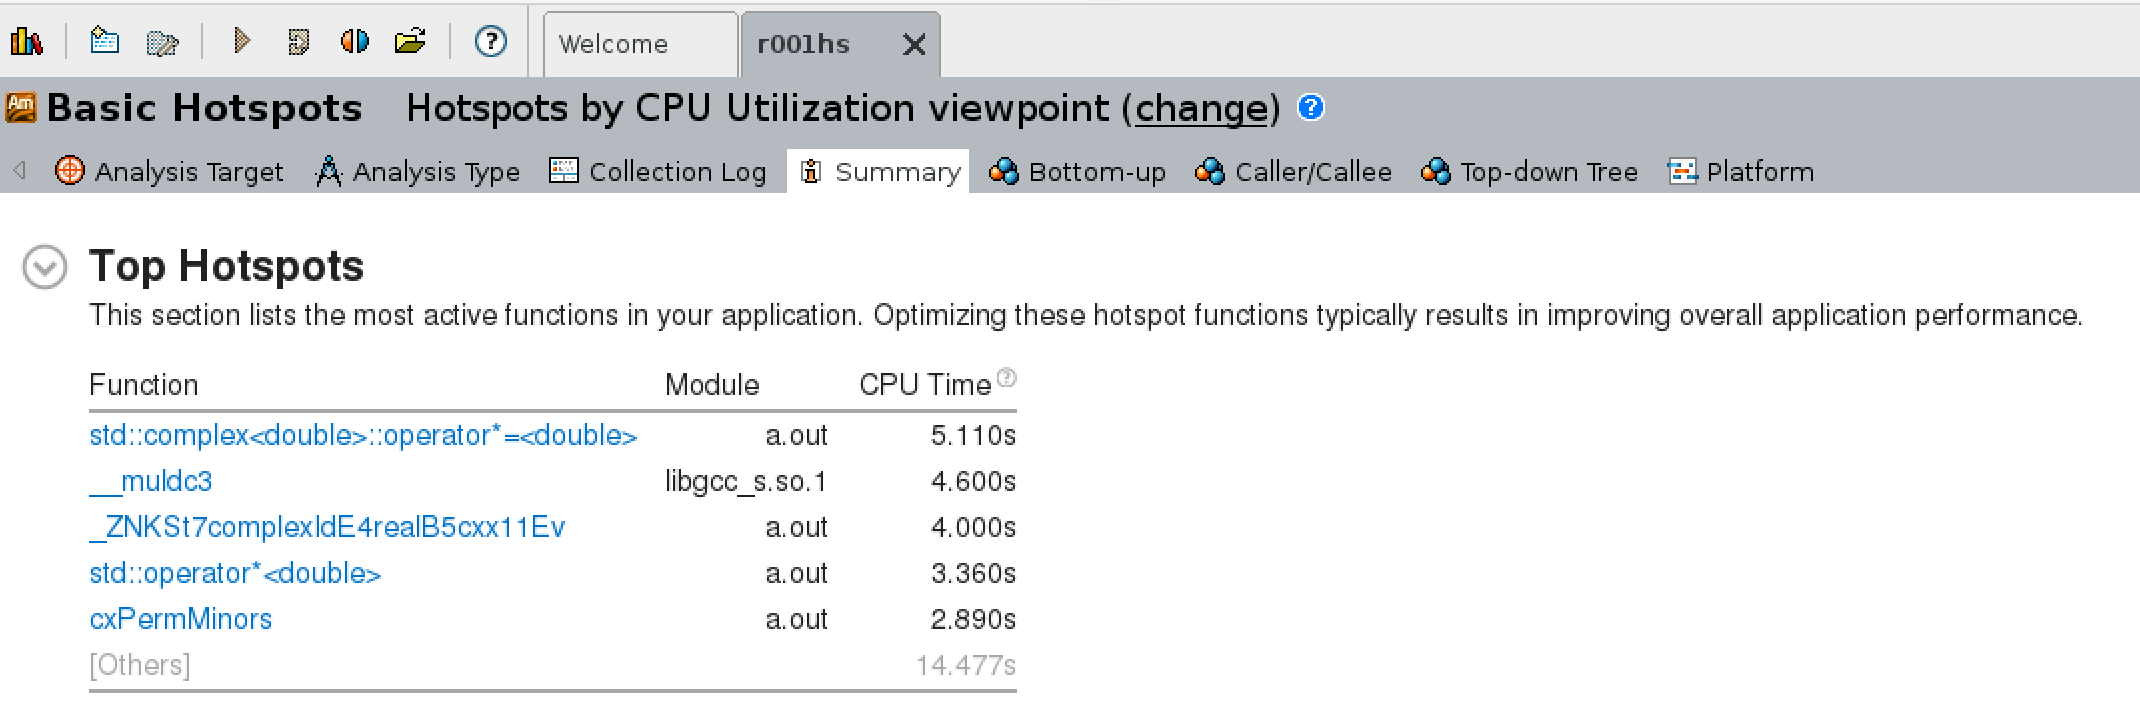
\includegraphics[width=\linewidth, frame]{vtune_hotspots_initial.png}}
  \caption{A summary of `hotspots' in the code identified by the Intel Vtune Profiler}
  \label{fig:vtune_hotspots_initial}
\end{figure}
The top 4 `hotspots' identified were all related to the operation of multiplying two objects of type \mintinline{c++}{std::complex<double>}. The Bottom-Up representation showed that the top 4 hotspots were all within the \mintinline{c++}{for} loop of \mintinline{c++}{cxPermMinors( ... )}, which is exactly as expected since the runtime of the algorithm is dominated by the loop required for computing the permanent minors.

Note that the second hotspot `\_\_muldc3' is an internal library routine, which is run by the C\texttt{++} compiler when two complex numbers are multiplied. To see this, I used the online tool Godbolt \cite{god-bolt} (Section \ref{sec:godbolt} which converts high-level code in some programming language (C\texttt{++} in our case) to low-level, compiler-dependent assembly code that. This showed that in assembly-level language, the g\texttt{++} compiler basically replaced lines containing the multiplication of two complex numbers with a list of instructions, one of which was a call to `\_\_muldc3'. Complex multiplication is a fairly straightforward operation that can be simplified as follows,
\begin{equation}
(a + bi) * (c+di) = (ac - bd) + (ad + bc)i
\end{equation}
which is an operation that one would expect to be calculated very efficiently in C\texttt{++} since it is reduced to a few simple arithmetic calculations on real numbers. However, an open-source implementation of `\_\_muldc3' \cite{muldc3} shows that the function is much larger than expected, due to a number of checks being made for edge cases on complex numbers. This is another bottleneck that could potentially be resolved. The third hotspot is simply a mangled name for an internal library routine that deals with complex numbers in C\texttt{++} and is called by `\_\_muldc3'.

To avoid having to run the profiler every single time, a timer function was added into the code to keep track of how long the entire program takes to run, as well as the cumulative runtime of the \mintinline{c++}{cxPermMinors(...)} function.
\begin{minted}[frame=lines,framesep=8pt]{c++}
auto start = chrono::steady_clock::now();
... 
int totalTime = chrono::duration_cast<chrono::milliseconds>(end - start).count();
\end{minted}

\section{Parallelising the code}
\subsection{Parallelisation technique}
The most obvious solution to speed up the process of calculating the permanent minors is to parallelise Lines 6 to 11 of the algorithm. This corresponds to the \mintinline{c++}{for} loop in the code which iterates over the values of $\delta$. For an input matrix of size $n \times n-1$, there are $(2^{n-1} -1)$ iterations of the loop. As $n$ grows, this number grows exponentially, so making the iterations run in parallel would have a significant impact. The reason that the loop is in fact parallelisable is that its purpose is essentially to generate some values in each iteration and add them to an accumulator. In order to parallelise it, each thread would have to maintain its own local accumulator, and the total number of iterations could be divided equally among the threads. After each thread completes its assigned set of iterations, it would add the values in its local accumulator to a global accumulator, which would finally hold the required end result. However, this was not as trivial as it sounds since a number of variables within the loop were dependent on their values in the previous iteration. Hence, we needed to find a way to initialise these variables to the correct values for any iteration number, so that a thread could be given these starting values before running its set of iterations. The modifications made for this parallelisation to work are explained in this section.

\paragraph{a) Getting the value of the active index $j$ in the $k^{\text{th}}$ iteration:} The loop in the original code iterates over $\delta$ in Gray code order by keeping track of the `active index' $j$ and then flipping the $j^{\text{th}}$ bit of $\delta$ at the end of each loop iteration. This active index $j$ is also required for calculating successive values of the vector $\mathbf{v}$, so it was also essential to derive a method for finding the value of $j$ in the $k^{\text{th}}$ iteration. To see how the value of $j$ relates to the iteration number $k$, refer to Table \ref{tab:graycode}. Notice that $j$ is equal to the position of the least significant bit set to 0 in the binary representation for $k$. Equivalently, it is the number of of trailing 0-bits in $j+1$, starting at the least significant bit position. There exists an intrinsic function (or built-in function) which does this exact operation for us. Intrinsics are a special collection of functions which are handled directly by the compiler, and are mapped directly to x86 SIMD(Single instruction, multiple data) instructions. Since these intrinsics are nearly equivalent to directly using actual assembly code, they are also highly efficient. For example, the corresponding intrinsic in the g\texttt{++} compiler is \mintinline{c++}{__builtin_ctzll (unsigned long long)}. Using this function in each iteration of the loop also allows us to get rid of the auxiliary array \mintinline{c++}{g} in the original code. it is used in the following way:
\begin{minted}[frame=lines,framesep=8pt]{c++}
int getActiveIndex(long long ctr) {
	return __builtin_ctzll(ctr);
	// _mm_tzcnt_64 for intel compiler
}
...
for (...) {
    ...
    j = getActiveIndex(ctr+1);
}
\end{minted}

\paragraph{b) Getting the value of $k^{\text{th}}$ element of the Gray code:} Once we have the correct values of $j$ in each iteration of the loop, we can use it as before to iterate from one element in the Gray code to the next in the same way as in the original implementation. However, if a thread is made to start from the $k^{\text{th}}$ iteration, it also needs to be assigned an initial value for $\delta$. Once again, refer to the example in Table \ref{tab:graycode} to see how elements of the Gray code are related to iteration number $k$. Notice that the Gray code corresponding to index $j$ is actually equal to $j \text{ XOR } j >> 1$ where $j >> 1$ represents a single bit shift to the right. Additionally, integer representation of the Gray code element is required to be converted to the $\delta$ representation, where 1s in the Gray code are represented by 0s in $\delta$ and 0s in the Gray code are represented by 1s. The functions for these operations are called by each thread right before it starts its loop iterations.
\begin{minted}[frame=lines,framesep=8pt]{c++}
int getKthGrayCode(long long k) {
    return k ^ (k >> 1);
}
\end{minted}

\paragraph{c) Getting the value of \mintinline{c++}{s}:} Recall that \mintinline{c++}{s} was a boolean variable which decided whether partial products would be added or subtracted to the accumulator. Since in the original serial code, the value of $s$ alternated between true and false across iterations, we use the fact that for an even iteration number, \mintinline{c++}{s} was set to \mintinline{c++}{false} and for odd iterations, \mintinline{c++}{true}. This needs to be done only once for each thread, as the value of \mintinline{c++}{s} could simply be flipped at the end of each iteration to update the value correctly.
\begin{minted}[frame=lines,framesep=8pt]{c++}
//my_start is the starting index for a thread
if (my_start%2 == 0) s = false;
		else s = true;
\end{minted}

\paragraph{d) Computing the $\mathbf{v}$ array for iteration $k$:} Computing the value of $\mathbf{v}$ for a given $\delta$ requires a direct interpretation of the formula $v_i (\delta) = \sum_{j=1}^{m-1} \delta_j b_{ji}$ from the equation for calculating permanent minors (Equation \ref{eq:permMinors}. Once again, this only needs to be done once for each thread since we use a different and more efficient method to iterate from one value of $\mathbf{v}$ to the next, which was described in section \ref{sec:permMinors}.
\begin{minted}[frame=lines,framesep=8pt]{c++}
arma::cx_vec getV(arma::uvec d, int j, int n, long long ctr, arma::cx_mat C) {
    arma::cx_vec v(n);
    v = arma::sum(C,1)/2;
    for (int i = 0; i < n; i++) {
        if(d[i] == 0) v -= C.col(i);
    }
    ...
    return v;
}
\end{minted}

\begin{table}
  \begin{center}
    \caption{Elements of Gray code and active indices for $n = 4$}
    \label{tab:graycode}
    \begin{tabular}{|c|c|c|c|}
    \hline
      \textbf{Iteration number} & $k$ \textbf{in binary} & \textbf{Active index} & \textbf{Gray code elements}\\
      $k$ & & $j$ & $\delta$\\
      \hline
      0 & 000 & 0 & 000 \\
      1 & 001 & 1 & 001 \\
      2 & 010 & 0 & 011 \\
      3 & 011 & 2 & 010 \\
      4 & 100 & 0 & 110 \\
      5 & 101 & 1 & 100 \\
      6 & 110 & 0 & 101 \\
      7 & 111 & 3 & 111 \\
      \hline
    \end{tabular}
  \end{center}
\end{table}

Using these techniques, I was able to parallelise the code with the help of OpenMP.

\subsection{Using OpenMP to modify the code for use with multiple threads}
The code was parallelised using OpenMP pragmas (Section \ref{sec:openMP}). The loop was converted from a `while' loop to a `for' loop, since the number of iterations is known to us. In addition, instead of carrying out the first iteration before the loop and then running the loop for $2^{n-1} -1$ iterations, the loop is made to run for a collective total of $2^{n-1}$ iterations. The task was to divide the iterations between threads as efficiently as possible.

Consider the case where the number of threads is equal to a multiple of 2. In this case, dividing the iterations between the threads is fairly straightforward. The threads are indexed $0 ... t-1$, if there are $t$ threads being used. The starting loop index for each thread is defined by the following formula:
\begin{equation}
\text{Start Index} = \frac{2^{n-1}}{t} * \text{threadIndex}
\end{equation}
and similarly, the ending loop index for a thread is calculated in the following way
\begin{equation}
\text{End Index} = \frac{2^{n-1}}{t} * (\text{threadIndex} + 1).
\end{equation}
Hence, each thread runs $ {2^{n-1}}/{t} $ loop iterations.

However, in the case that the number of threads is not a power of 2, the iterations are not divided equally among all threads but we do ensure that they are divided in such a way that each thread has no more than 1 extra iteration compared to any other thread. This is done with a slight modification on the formulas above, where the if there are $x$ extra iterations, the first $x$ threads get $\text{floor}( {2^{n-1}}/{t} ) + 1$ iterations.

Threads are created using the \mintinline{c++}{pragma omp parallel} construct, and then the start and end index of the loop is defined for each thread, Along with this, the number of threads, and scope of variables is specified in the \mintinline{c++}{pragma}. This \mintinline{c++}{pragma} is used to actually create a team of \mintinline{c++}{numThreads} threads, and the only variables shared across threads are the input matrix, and the global accumulator. The rest of the variables are made thread local as they are modified by each thread individually at the same time. 
\begin{minted}[frame=lines,framesep=8pt]{c++}
#pragma omp parallel num_threads(numThreads) private(d, v, s, q, j) shared(C, p)
{
    ...
}
\end{minted}
The variables local to the loop are initialised to the appropriate values, and then the loop is run. Finally, the local accumulator is added to the global accumulator using the \mintinline{c++}{pragma omp critical} construct. This construct specifies that the code is to only be executed on one thread at a time.
\begin{minted}[frame=lines,framesep=8pt]{c++}
#pragma omp critical
{
    p+= p_local;
}
\end{minted}
With this, the code was parallelised to the standard I had aimed for. Checks were run on the code and it was tested against known values of permanents of matrices to ensure correctness. Refer to Appendix \ref:{app:code} for the code of the functions described.

\section{Other Optimisations}
\subsection{Compiler choice}
The execution time of the code is determined by the number of instructions that the CPU executes. Since the compiler is responsible for translating our high-level C\texttt{++} code to a set of low-level assembly instructions, the choice of compiler can have a significant effect on performance. I tested the code with two different compilers: the g\texttt{++} compiler by GCC, and the Intel C\texttt{++} compiler, both of which provide support for OpenMP.
\paragraph{GCC g\texttt{++} compiler: } GCC (or GNU Compiler Collection) actually refers to a collection of compilers for different programming languages, and is widely used especially for C\texttt{++}. The version we use is GCC 7.2. g\texttt{++} is a portable, multi-platform compiler and can produce outputs for most types of processors. It is a free software, distributed under the GNU General Public License \cite{gcc_compiler}.

\paragraph{Intel C\texttt{++} compiler: } The Intel C\texttt{++} compiler is a highly optimised compiler for systems using processors that support Intel architectures. The Intel compiler automatically performs operations such as Single Instruction Multiple Data vectorisation, which speeds up standard operations by performing them simultaneously using the processors hardware. In addition, it also carries out loop and memory transformations to speed up a program. The only caveat is that it may not carry out these intensive optimisations for systems without Intel architectures. It is freely available for students, educators and open-source developers \cite{intel_compiler}.

Since one was not clearly better than the other, I used both at every stage of testing to compare results.

\subsection{Compiler options} \label{sec:flags}
Both compilers offer useful optimisation options, which we test on our program as well. Compiler options are not required to compile the program, but they do provide the ability to change how the code is processed by the compiler. The options we tested are summarised in the following tables \cite{gcc_flags}.

\begin{table}[h!]
\centering
	\begin{tabular}{ |p{0.25\textwidth} | p{0.75\textwidth} |}
    	\hline
	\textbf{Option} & \textbf{Notes} \\
   	\hline
	\mintinline{console}{-Ofast} & Flags beginning with \mintinline{console}{-O} enable a number of different optimisation options. \mintinline{console}{-Ofast} actually combines  \mintinline{console}{-O3}, which provides the highest level of optimisations and \mintinline{console}{-ffast-math}, which tells the compiler to ignore a number of IEEE or ISO rules/specifications for some math functions. Hence, this may speed up code greatly, but is not always safe to use.\\
	\hline
	\mintinline{console}{-march=native} & This tells the compiler what exact code it should produce for the systems processor architecture, since different CPUs support different instruction sets.\\
	\hline
	\mintinline{console}{-funroll-loops} & Unrolls loops whose number of iterations can be determined at compile time or entry to the loop. This option does make the code larger, and may or may not speed up the code.\\
	\hline
	\mintinline{console}{-pipe} & Has no effect on the generated code, but it speeds up the compilation process.\\
	\hline
	 \end{tabular}
\caption{Compiler options used with the g\texttt{++} compiler} \label{tab:gcc_compiler_flags}
\end{table}

\begin{table}[h!]
\centering
	\begin{tabular}{ |p{0.25\textwidth} | p{0.75\textwidth} |}
    	\hline
	\textbf{Option} & \textbf{Notes} \\
   	\hline
	\mintinline{console}{-O3} & Flags beginning with \mintinline{console}{-O} enable a number of different optimisation options. \mintinline{console}{-O3} provides the highest level of optimisation by enabling compiler vectorisation, and aggressive loop transformations among other techniques.\\
	\hline
	\mintinline{console}{-xHOST} & This tells the compiler what exact code it should produce for the systems processor architecture, since different CPUs support different instruction sets.\\
	\hline
	 \end{tabular}
\caption{Compiler options used with the Intel C\texttt{++} compiler} \label{tab:intel_compiler_flags}
\end{table}

The effects of using compiler options varies greatly from system to system, and his highly dependent on the code, so I compiled the program with various combinations of these options to see how they would affect the results.
\\
\\
\\
The code implementation explained in this chapter, even before parallelisation is already a much more efficient implementation than most previous attempts since it implements the new and improved algorithm with optimisation in mind. Algorithm B already provides a dramatic speed up over the naive algorithm, and the parallelised implementation should, in theory make it even more efficient. The code was tested out and the results described in the next section.
% -----------------------------------------------------------------------------

\chapter{Critical Evaluation}
\label{chap:evaluation}

I tested out the above implementation at each stage on BC4 and recorded the timings. In order to provide a clear comparison of the features used, and how they affected runtime, I carried out tests at each stage of the development and compared the different optimisations made individually, and together.


\section{Initial implementation}
I first tested out the C\texttt{++} code without any optimisations made, compiled with both the Intel and g\texttt{++} compilers. This has been plotted as a graph shown in figure \ref{fig:org}. For each value of $n$ from 2 to 30, 10 results were recorded, with their timing taken. The mean and standard deviation of the code runtimes for each of these values was calculated and is depicted in the graph. The error bars represent one standard deviation in the data. Notice that the y-axis of the graph uses a log-scale, which is why the lines appear to be roughly linear. Since the time taken was expected to grow exponentially from the theoretical runtime of Algorithm B, the observed results matched the theoretical ones. 

The Intel compiled code was significantly faster than the g\texttt{++} compiled code. The average time for the g\texttt{++} compiled code to complete the algorithm was $\approx1100$ seconds, whereas for the Intel compiled code, it was $\approx100$ seconds. The probable reason that the Intel compiled code is over 10 times faster is that it is highly optimised by the compiler even without specifying any additional optimisation options.

Additionally, we can see that the time taken for computation of permanents is consistently only a little bit less than the total time taken, except for smaller values of $n$. For small values of $n$ less than 13 and 16, with the g\texttt{++} and Intel compilers respectively, the amount of time taken to compute permanents was 0. This is because for small sizes of matrices, calculating the permanents does not require too many steps. The overheads of running the rest of the algorithm appears to dominate for these small values of $n$. However, as $n$ increases, the time spent in computing permanents increases sharply, and accounts for most of the total run time, as the exponential growth in time does after all come from the calculation of permanents.

It was also interesting to note that the timings to run the Intel compiled code were a lot more consistent than the timings for the gcc compiled code. The standard deviation for the g\texttt{++} code with higher values of $n$ was roughly 130, whereas for Intel, it never exceeded 0.8, giving the coefficients of variation 11\% and 0.8\% respectively. This is probably an effect of the optimisation steps by the Intel compiler that cause it to give consistent results each time.
\begin{figure}
	\centering
  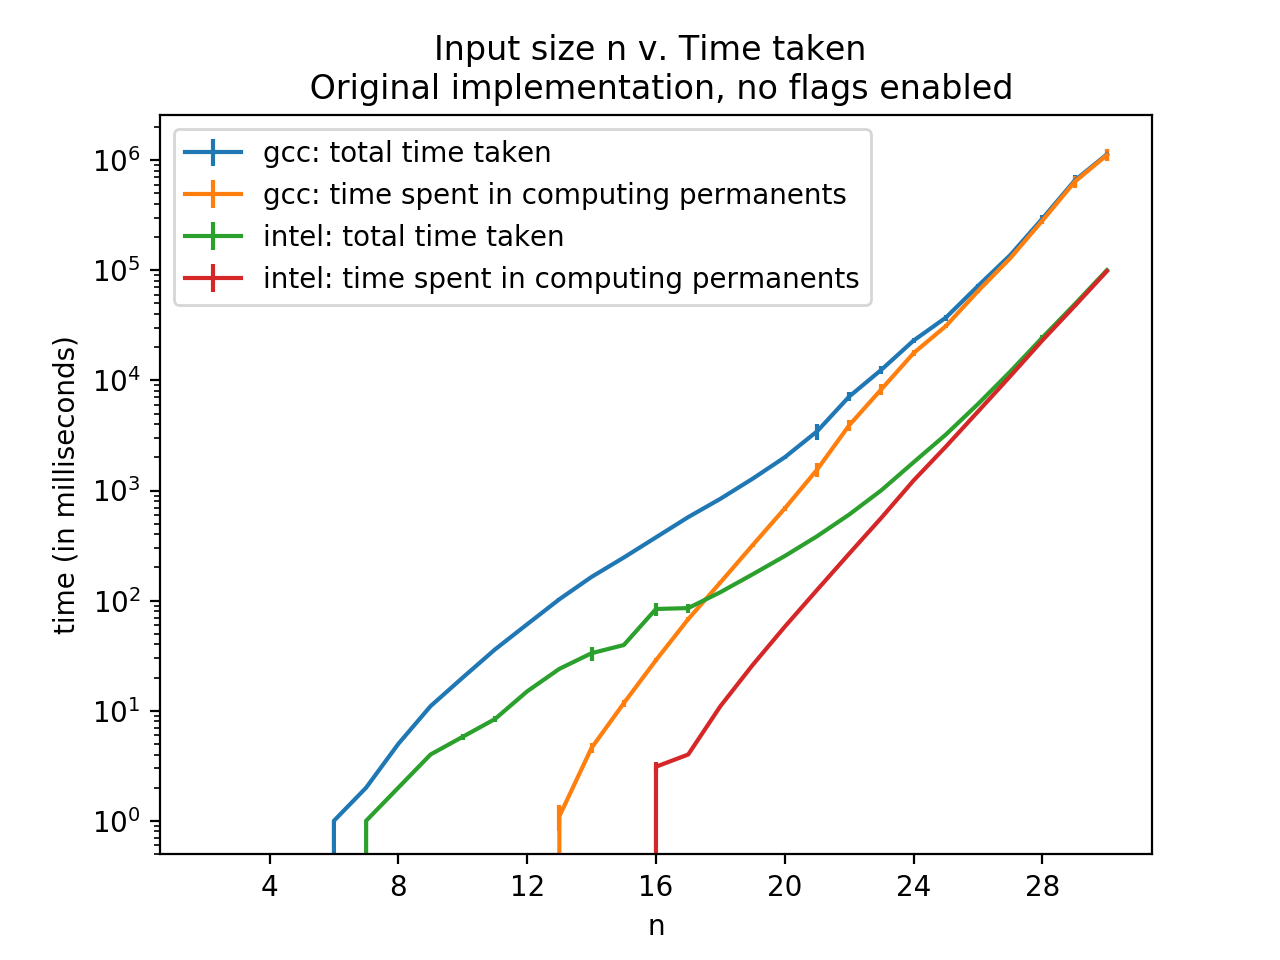
\includegraphics[width=25em]{Graphs/org_log.png}
  \caption{Original implementations}
  \label{fig:org}
\end{figure}

\section{Testing the different compiler options/flags}
After parallelising the code, in order to compare the different compiler options, the code was run on 16 cores with different options enabled each time. As before, 10 samples were taken for each value of $n$, and the means are plotted in the graphs.
\subsection{g\texttt{++}}
We had four different compiler options to test with g\texttt{++}, as explained in section \ref{sec:flags}, and the results are shown in figure \ref{fig:gcc_flags}. The \mintinline{console}{-funroll} option makes almost no difference, which I had anticipated since it is known to not improve timings in many cases. Specifically, in the case of our loop which was run an exponential number of times for permanent calculation, unrolling loops would potentially make the process of going from one iteration to the next faster, but a lot more memory would be used as a cost, which would slow it back down. 

What was more surprising was that the \mintinline{console}{-march=native} flag had only a minute effect (1 to 2 seconds for n=30) in speeding up the time. I tested the code on a personal computer as well with and without the  \mintinline{console}{-march=native} flag enabled. Surprisingly the difference in timings were a lot more noticeable as compared to the test on BC4. The tests on my computer showed a speed up of 15-20\%, while all BC4, the speed improvement was under 5\%. The effects of this flag are dependent on the hardware of the processor, which explains the difference between the results on BC4 versus the personal computer. A possibility is that the compiler on BC4 is that the exact processor hardware is already specified to the compiler in which case, I would expect the flag to have no noticeable effects.

On the other hand, the \mintinline{console}{-Ofast} flag provided a major speed up, making the code over 10 times faster to run than with no compiler options enabled. The code was profiled again at this stage to understand how such a significant speed up was made and the results are shown in figure \ref{fig:vtune_Ofast}. The difference is that the top few hotspots are no longer dominated by the inbuilt function `\_\_muldc3', and other specific operations related to multiplying complex numbers. The reason this has happened is that using \mintinline{console}{-Ofast} tells the compiler to ignore strict ISO standards, and instead of running the complex number multiplication function with a lot of checks, it simply performs the bare operations. While it does make the code susceptible to errors in edge cases (specifically involving operations where the real part of the number is set to infinity), I expect to never encounter these cases in the code, and can ensure that I don't by adding in some checks of my own.

\begin{figure}
	\centering
  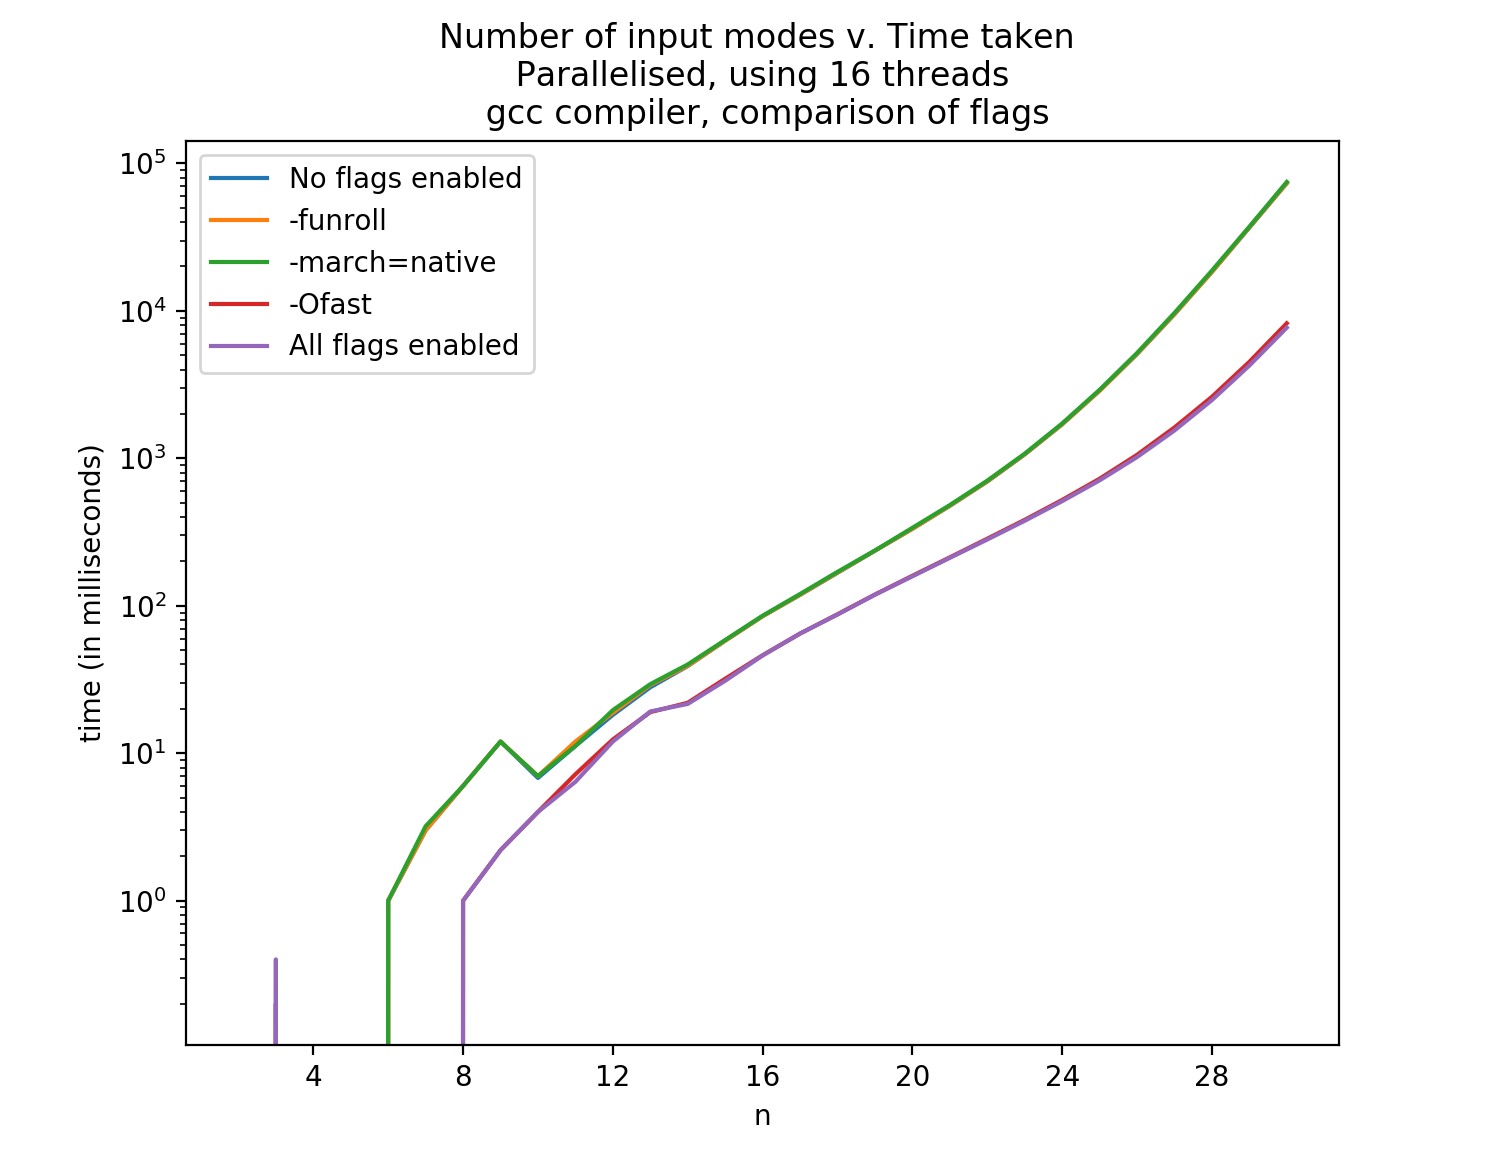
\includegraphics[width=25em]{Graphs/gcc_flags_log.png}
  \caption{Comparing different g\texttt{++} compiler options}
  \label{fig:gcc_flags}
\end{figure}

\begin{figure}
	\centering
  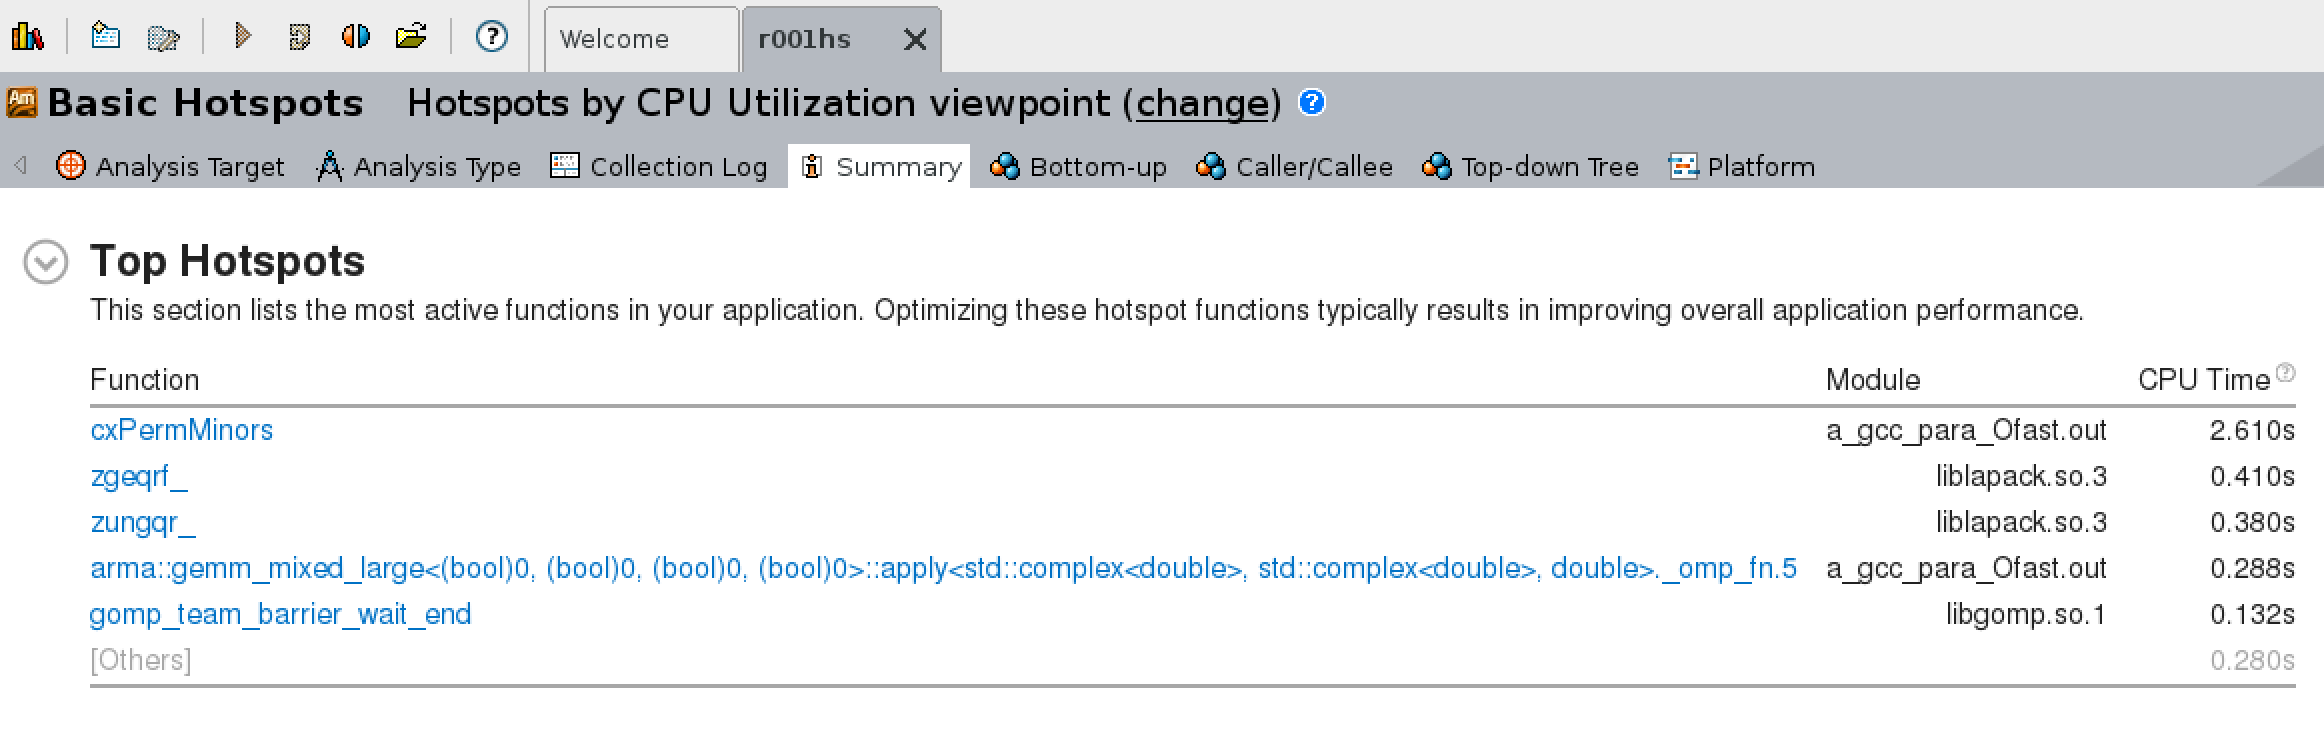
\includegraphics[width=\textwidth, frame]{vtune_hotspots_Ofast.png}
  \caption{A summary of hotspots found in the code identified by the Intel Vtune Profiler after enabling the -Ofast flag}
  \label{fig:vtune_Ofast}
\end{figure}

\subsection{Intel compiler}
The two chosen flags were tested on the Intel compiler and disappointingly, neither of the two made a big difference to the timing. This is shown in figure \ref{fig:intel_flags}. Considering how much faster the Intel compiled code was even before any options were added, that the added optimisations would not have any effect on the specific operation used in my code. I verified this by profiling the code, and noticed that using the optimisation flags does sharply reduce the time for some matrix operations, these were operations that only accounted for a small fraction of the total time, which is why the difference is not noticeable.
\begin{figure}
	\centering
  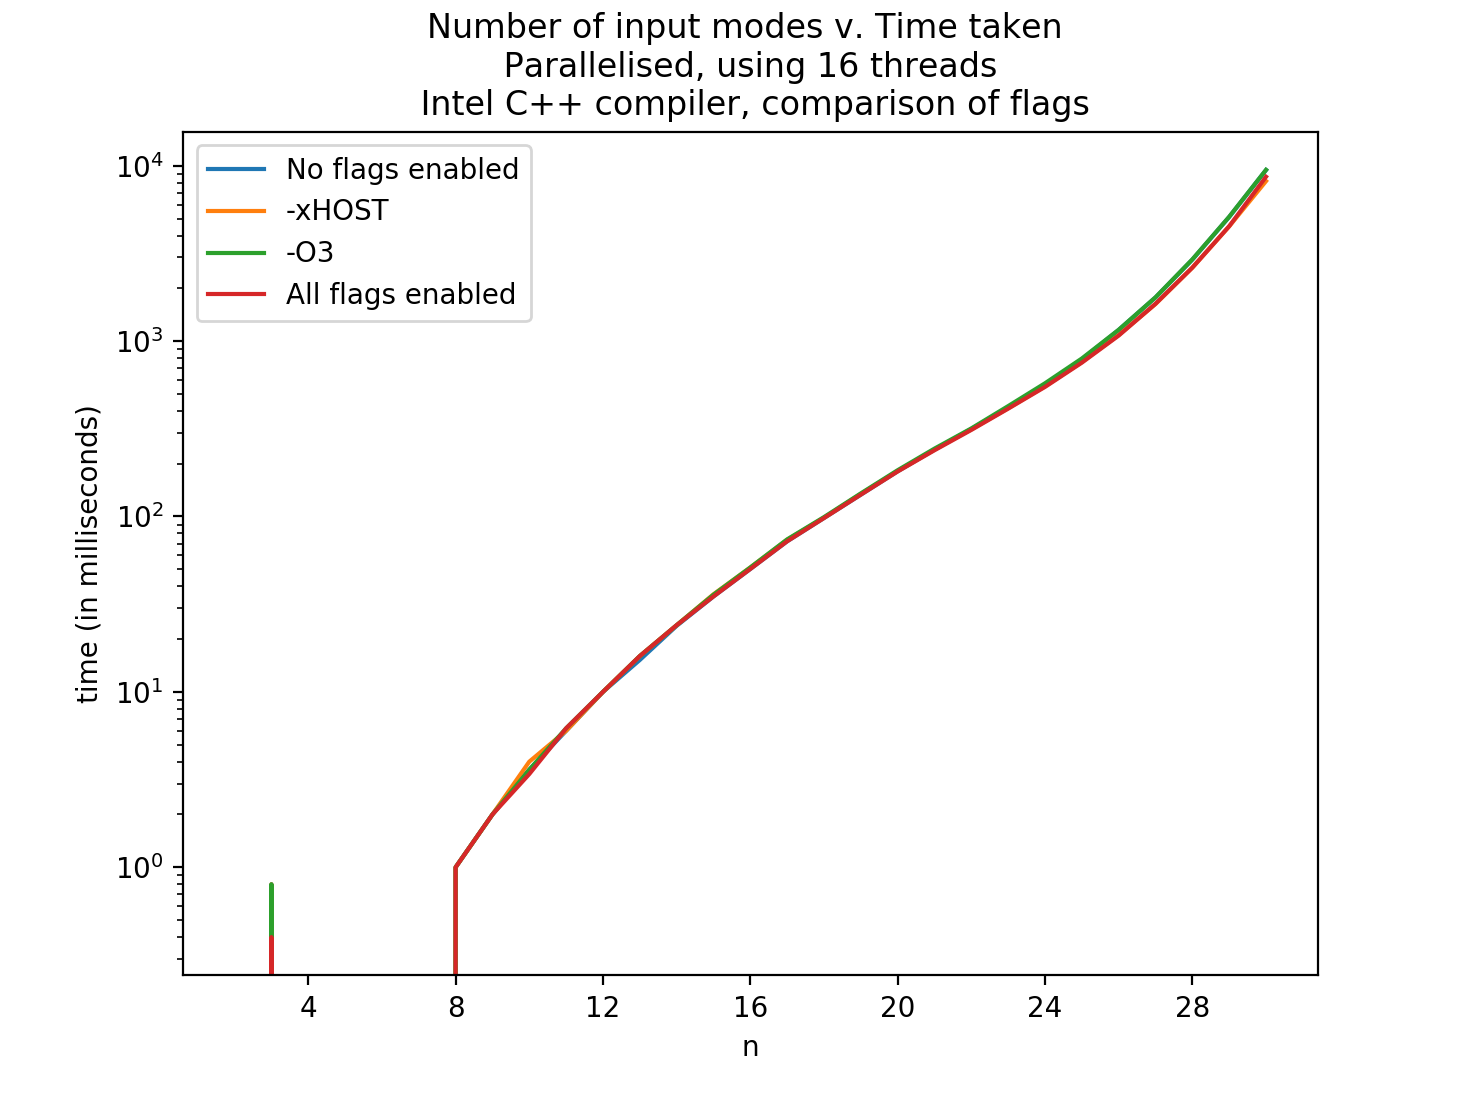
\includegraphics[width=25em]{Graphs/intel_flags_log.png}
  \caption{Comparing different Intel compiler options}
  \label{fig:intel_flags}
\end{figure}

After enabling optimisation flags, the g\texttt{++} and Intel compiled code have similar timings for $n=30$, with the g\texttt{++} compiled code occasionally being 1-2 seconds faster.

\section{Multiple threads}
One of the main aims of this project was to parallelise the algorithm, and the results obtained by doing so were as expected. The code was run after being compiled with both compilers and all listed flags enabled, with a different number of threads available each time for the sake of comparison. The results obtained showed a speed up roughly proportional to the number of threads used, shown in figures \ref{fig:gcc_threads} and \ref{fig:intel_threads}. 

In a few cases for values between $n=8$ and $n=12$, we can see that in figure \ref{fig:gcc_threads} there are some inconsistencies, and using more threads might take a few milliseconds more than with less threads. This is because multithreading does have overheads with assigning values to threads as well as with creating threads, and with smaller values of $n$ (and subsequently, less time used to carry out actual computation of the algorithm), these overheads become more obvious. 

There were no significant differences between the Intel compiled code and the g\texttt{++} compiled code.
\begin{figure}
	\centering
  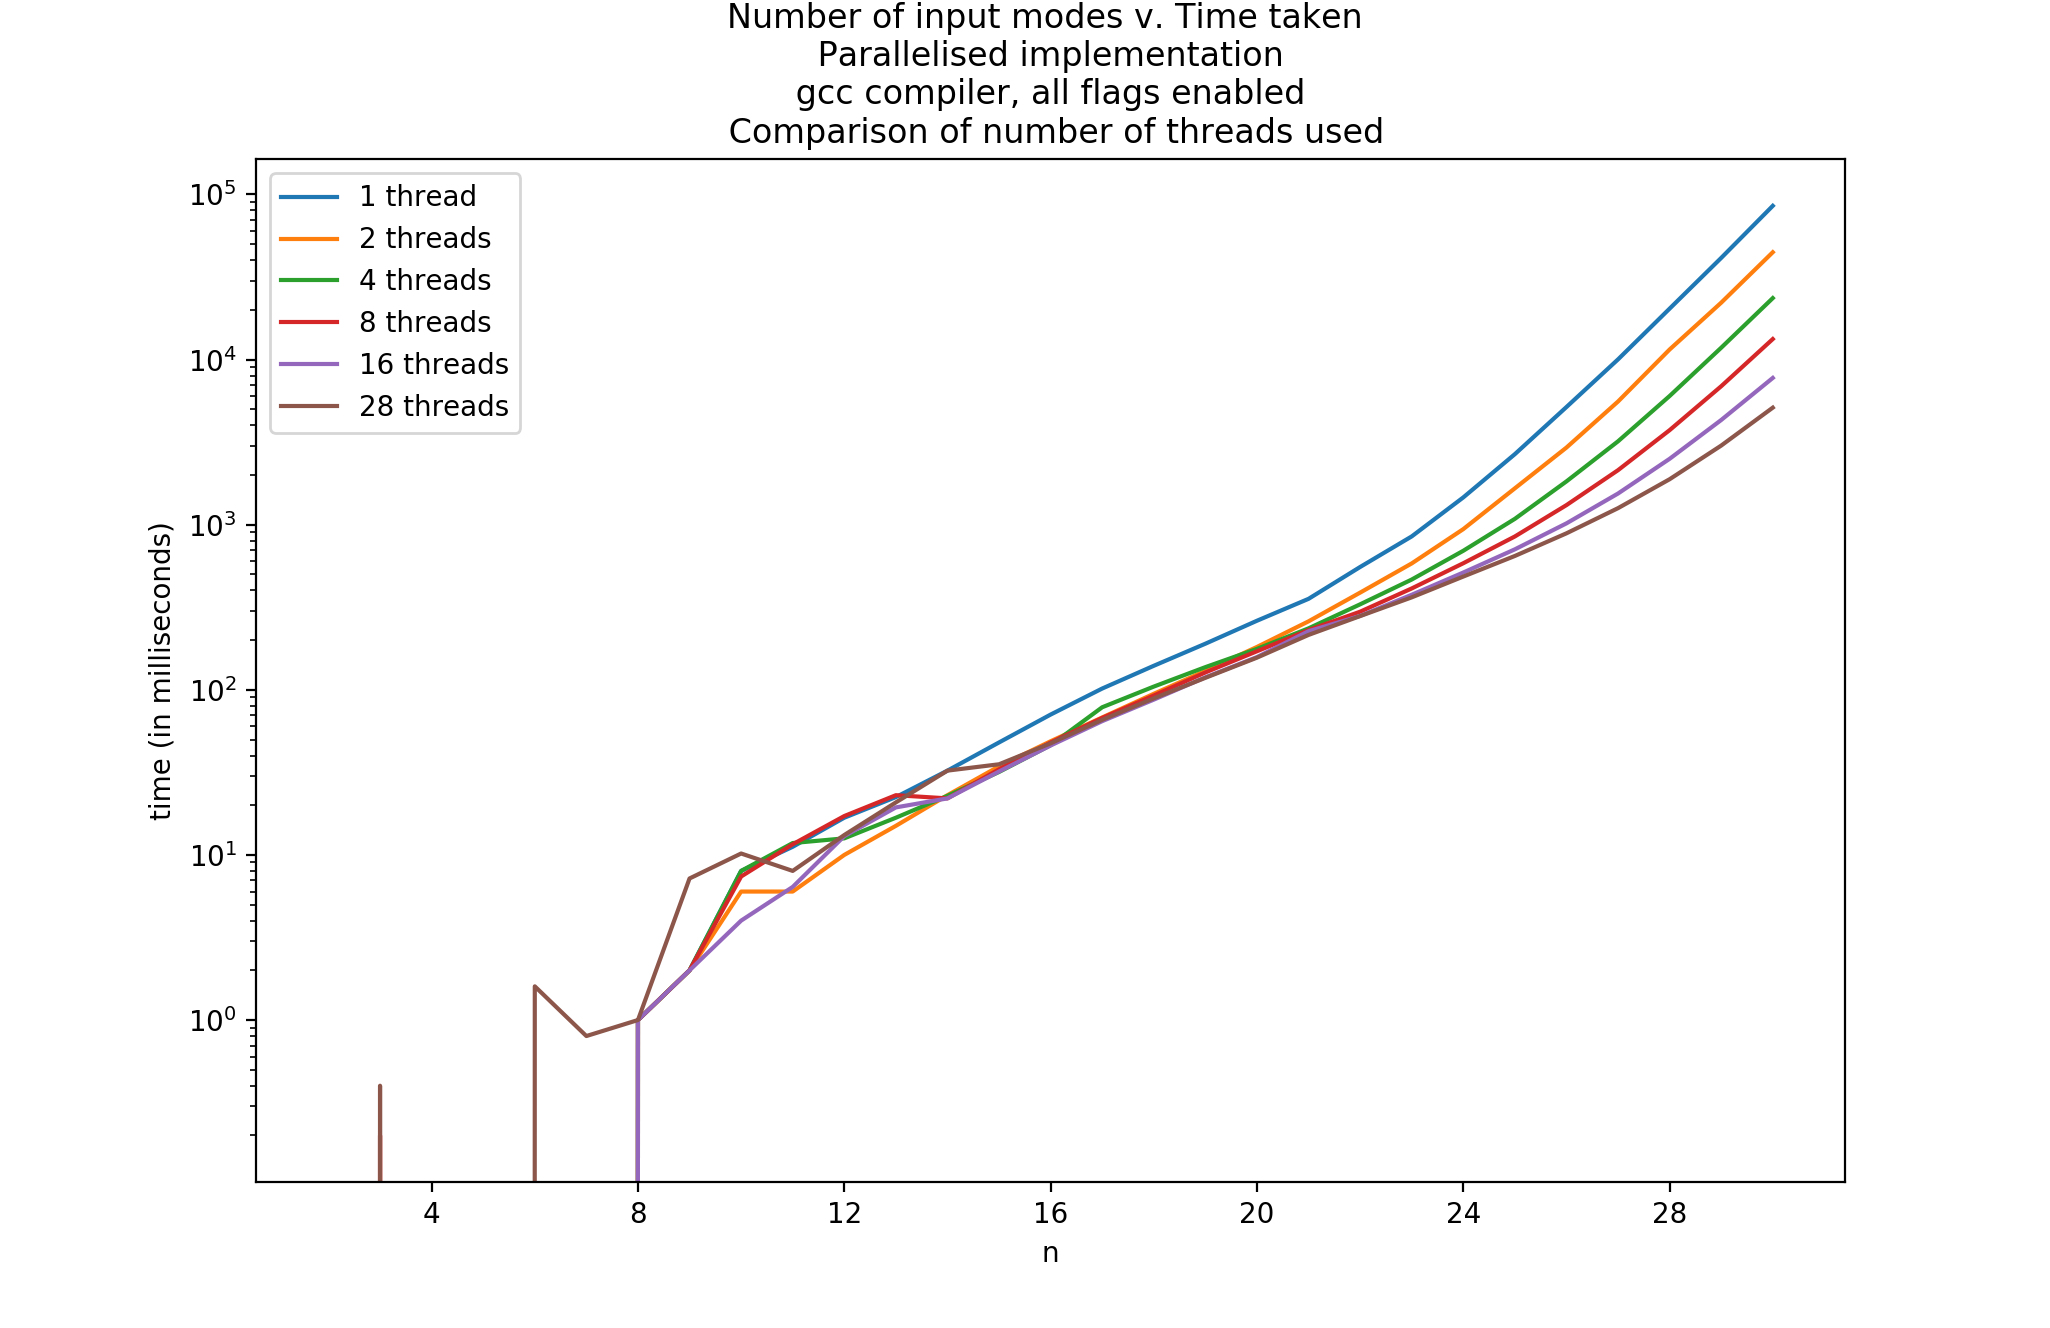
\includegraphics[width=25em]{Graphs/gcc_threads_log.png}
  \caption{Comparing different number of threads used with g\texttt{++} compiled code}
  \label{fig:gcc_threads}
\end{figure}

\begin{figure}
	\centering
  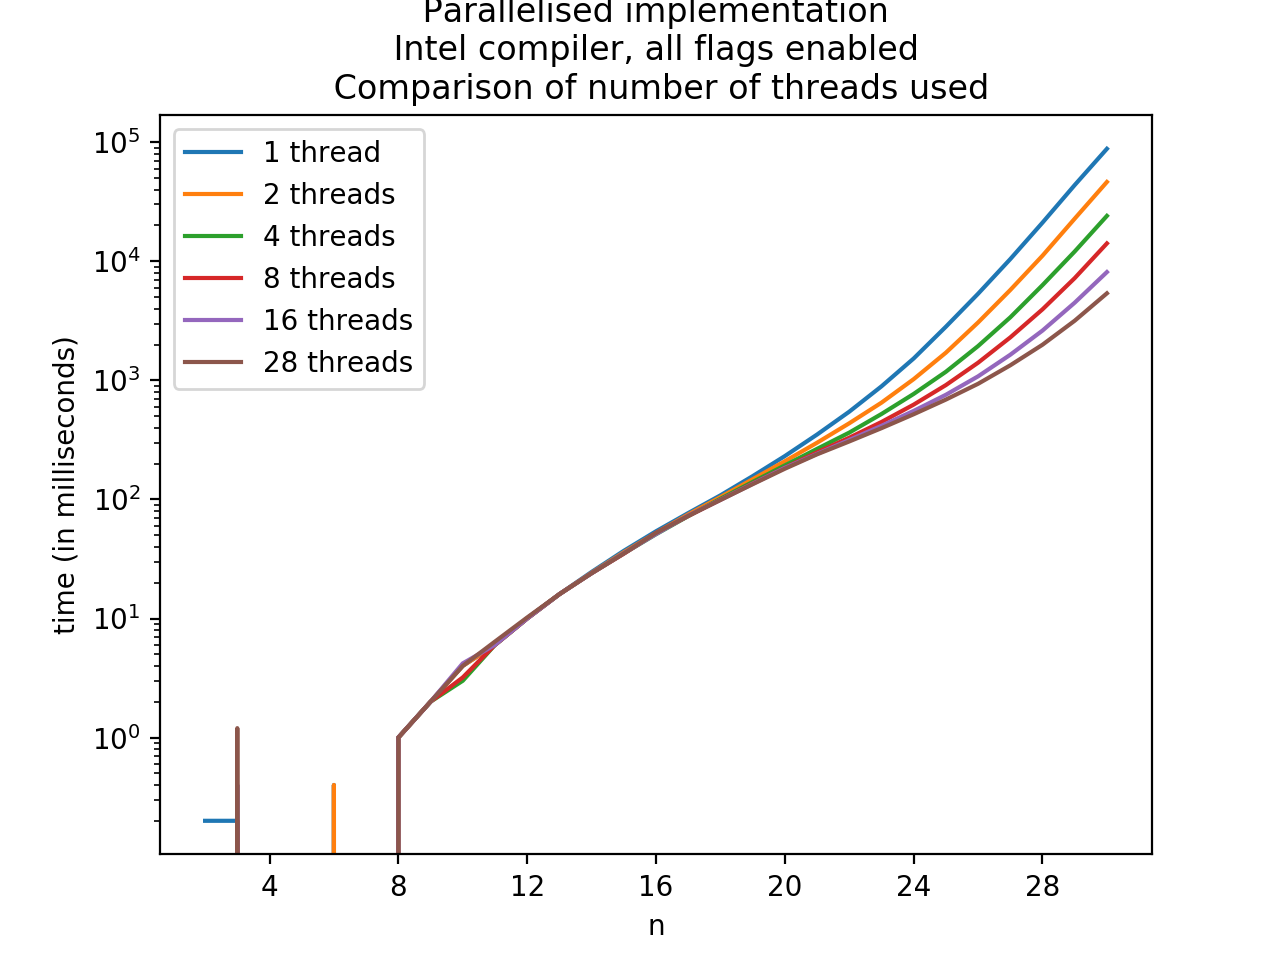
\includegraphics[width=25em]{Graphs/intel_threads_log.png}
  \caption{Comparing different number of threads used with intel compiled code}
  \label{fig:intel_threads}
\end{figure}

Another set of timings was taken for running the Boson Sampling code with $n=30$, and successively increasing the number of threads, shown in figure \ref{fig:threadCurve}. The results show that the timing reduces exponentially, which is exactly as expected.

One can also notice the trend that as the number of threads is doubled, the timing is roughly halved. A summary of the actual timings are also shown in table \ref{tab:threads} (figures rounded to the nearest second).
The reason it is not exactly halved each time is that the portion of code that is not parallelised adds a constant overhead each time, for a given value of $n$, when the number of threads is varied. Apart from that, the overheads added by OpenMP also make a small difference.
\begin{figure}
	\centering
  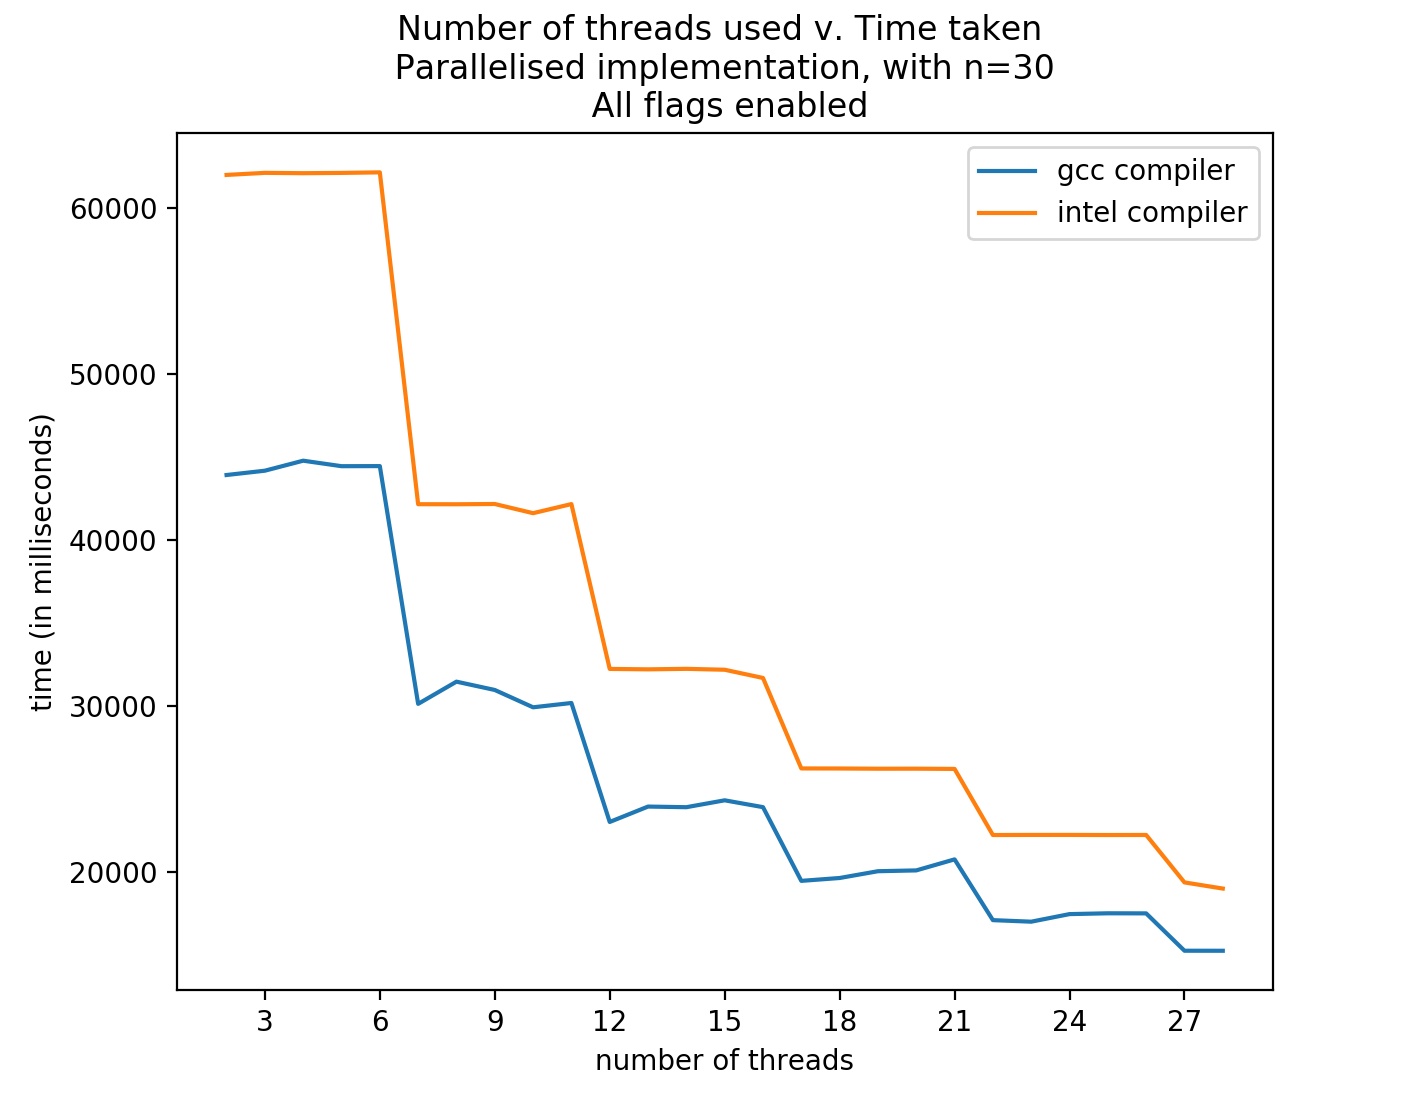
\includegraphics[width=25em]{Graphs/threadCurve_linear.png}
  \caption{Comparing different number of threads used}
  \label{fig:threadCurve}
\end{figure}

\begin{table}
  \begin{center}
    \caption{Timings to run code (in seconds), as number of threads is changed, for $n=30$}
    \label{tab:threads}
    \begin{tabular}{|c|cc|}
    \hline
      \textbf{No. of cores} & \textbf{Time for gcc} & \textbf{Time for Intel} \\
      \hline
      1 & 85 & 88 \\
      2 & 44 & 46  \\
      4 & 23 & 24 \\
      8 & 13 & 14 \\
      16 & 8 & 8 \\
      28 & 5 & 5 \\
      \hline
    \end{tabular}
  \end{center}
\end{table}

\section{Final result}
Using all the optimisations made, I ran the code on BC4, using 28 cores. The results are shown in \ref{fig:final_graph}. The g\textt{++} compiled code gives marginally faster results as compared to the Intel compiled code, and the times taken to simulate sampling bosons for $n=30$ are 5.1 seconds and 5.3 seconds respectively.
\begin{figure}
	\centering
  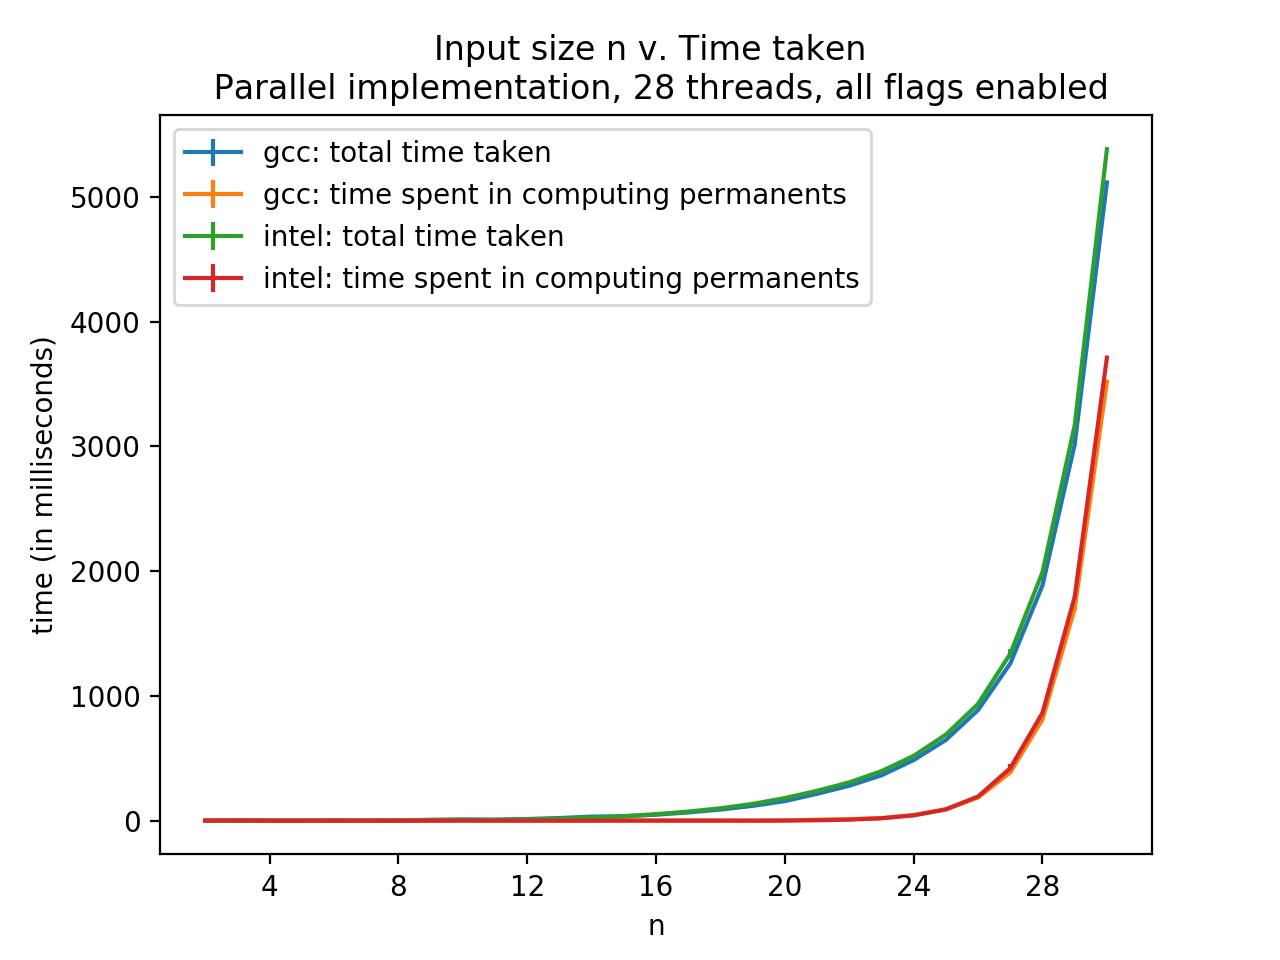
\includegraphics[width=25em]{Graphs/fastest_linear.png}
  \caption{Comparing final results}
  \label{fig:final_graph}
\end{figure}

One thing to note about the graphs the y-scale values are in logs, is that for small values of $n$, some spikes can be seen. This is expected as it is possible for overheads to vary by 15-20ms each time. In some of the graphs, the compiler mentioned is gcc. This is an error and should be read as g\textt{++}.
\\
\\
\\
The results obtained by the implementation I devised were as expected, and show promising results for the Boson Sampling problem as a whole.
% -----------------------------------------------------------------------------

\chapter{Conclusion}
\label{chap:conclusion}
\section{Achievements}
Apart from implementing the code, the purpose of this paper was to develop and demonstrate an understanding of the Boson Sampling problem from the perspective of classical computing. The explanations of the existing algorithms were summarised in Chapter \ref{chap:bosonSampling}, which lead the way for putting together a basic implementation of the algorithm. This was followed by the main aim of the project, which was to implement an optimised version of the Boson Sampling problem which I successfully carried out as described in Chapter \ref{chap:execution}. I explored different techniques for optimisation, the main one being the parallelisation of the function to calculate permanent minors. The parallel implementation used a number of different techniques that were not specific to the algorithm in order to ensure that it worked correctly and optimally. Apart from the parallelisation, I also ran tests to compare popular compilers and optimisation options. The results of the implementation were recorded at each stage and then compared and evaluated in the end.

The final results produced showed a speed up of around 200 times with the g\texttt{++} compiler, and 20 times for the Intel compiler, as compared to the initial measurements. I also ran a few tests for $n=35$, and it took approximately 320 seconds to run. While these numbers may not seem impressive compared to the benchmark on the Tianhe-2 supercomputer \cite{wu2018}, our implementation uses a maximum of 28 cores, whereas the benchmark for $n=50$ which was computed in 600 minutes was made using 312,000 cores. It is hard to see a direct comparison between these figures, but a more detailed explanation is given further down in Section \ref{sec:future}. I was initially aiming to try and reach this benchmark of $n=50$, but soon realised that with the optimisation techniques I had aimed to used, and with the hardware available to me, that this would not be feasible in the short term. Due to this limitation, I also did not manage to evaluate how well the implementation would work with larger values of $n$, in case affected issues such as memory overflow. Nonetheless, the speed up I was able to achieve was exactly as expected.

The implementation shown in this paper serves as proof to reduce the likelihood of near term quantum supremacy in the field of Boson Sampling, as was suggested by the authors of Algorithm B \cite{clifford17} and potentially raises the bar significantly for quantum research using linear optics.

\section{Future Works} \label{sec:future}
Since this implementation is one of the first few works of its kind, i.e. classically implementing Boson Sampling, it leaves a lot of scope for further work to be carried out. Primarily, the goal would be to introduce Multi-processing using a library like OpenMPI \cite{openmpi}. This would open up the possibilities of running the code on much larger systems as we would not be limited to the cores on a single processor. Using multiprocessing and running it on a large supercomputer are expected to give the desired results of setting a new benchmark for $n=50$. For the sake of comparison, I projected how much time it would take to run my implementation for $n=50$, using all the cores of the Tianhe-2 supercomputer, and estimate that it could take as little as 20 minutes, or perhaps even less. This figure was reached by multiplying my current results for $n=35$ by $2^{15}$, and then dividing it by the factor of extra cores that the supercomputer has. I made sure to allow for a significant amount error in this calculation as well to avoid overestimating a result.

In addition, other routes for optimisations can be made such as vectorisation, and using more low level code where possible. An interesting approach would be to use GPUs for the calculations which has the potential show highly positive results.

Finally, it is also important to guarantee correctness of the program, since it is meant to be an exact sampling algorithm. To resolve this, I could use a statistical testing technique such as the one proposed by Walschaers et. al \cite{2016NJPh...18c2001W} for Boson Sampling. It would also be useful to compare the results obtained (using the same random seed) with other established large-scale implementations.
\\
\\
\\
The Boson Sampling problem is one that has the potential to create a serious impact on quantum supremacy, either for or against it. Even though this paper has explored only a small part of the problem, it has been interesting to see how a powerful implementation of the algorithm could have strong implications against quantum supremacy.


% =============================================================================

% Finally, after the main matter, the back matter is specified.  This is
% typically populated with just the bibliography.  LaTeX deals with these
% in one of two ways, namely
%
% - inline, which roughly means the author specifies entries using the 
%   \bibitem macro and typesets them manually, or
% - using BiBTeX, which means entries are contained in a separate file
%   (which is essentially a databased) then inported; this is the 
%   approach used below, with the databased being dissertation.bib.
%
% Either way, the each entry has a key (or identifier) which can be used
% in the main matter to cite it, e.g., \cite{X}, \cite[Chapter 2}{Y}.

\backmatter

\bibliography{project_bib}

% -----------------------------------------------------------------------------

% The dissertation concludes with a set of (optional) appendicies; these are 
% the same as chapters in a sense, but once signaled as being appendicies via
% the associated macro, LaTeX manages them appropriatly.

\appendix

\chapter{Appendix A}
\label{app:code}
The code is available to access and test at: https://github.com/mananvaswani/classical-boson-sampling

In addition, the three main functions used are given here for reference:
\begin{minted}[frame=lines,framesep=8pt, label=Random Unitary Matrix]{c++}
#include "header.h"

arma::cx_mat randomUnitary(int m) {

    arma::mat A_real(m, m, arma::fill::randn);
    arma::mat A_imag(m, m, arma::fill::randn);

    arma::cx_mat A(A_real, A_imag);

    arma::cx_mat Q, R;
    arma::qr(Q, R, A);

    arma::mat R_diag = arma::sign(arma::real(arma::diagmat(R)));

    A = Q * R_diag;

    return A;
}
\end{minted}

\begin{minted}[frame=lines,framesep=8pt, label=Compute Complex Permanent Minors in Parallel, breaklines]{c++}
#include "header.h"

int getActiveIndex(long long ctr) {
	return __builtin_ctzll(ctr);
}

int getKthGrayCode(long long k) {
    //k--;
    return k ^ (k >> 1);
}

arma::uvec getDelta(long long ctr, int n) {
    int gray = getKthGrayCode(ctr);
    arma::uvec d(n);
    d.fill(1);
    // first flip the bits
    int temp = gray ^ (int)pow(2, n) - 1; // 2^(n) - 1
    int i = 0;
    while (temp != 0) {
        d[i++] = temp % 2;
        temp = temp / 2;
    }
    return d;
}

arma::cx_vec getV(arma::uvec d, int j, int n, long long ctr, arma::cx_mat C) {
	arma::cx_vec v(n);
	v = arma::sum(C,1)/2;
    for (int i = 0; i < n; i++) {
        if(d[i] == 0) v -= C.col(i);
    }
	if (ctr!=0) {
		if(d[j] == 1) v -= C.col(j); else v += C.col(j);
	}
    return v;
}

void printArmaVector(arma::uvec d) {
    for (int i = 0; i < d.size(); i++) {
        cout << d[i] << " ";
    }
    cout << endl;
}

void printArmaVector(arma::cx_vec d) {
    for (int i = 0; i < d.size(); i++) {
        cout << d[i] << " ";
    }
    cout << endl;
}

arma::cx_vec cxPermMinorsThreads(arma::cx_mat C, int numThreads) {
// Declarations
	int n = C.n_cols, m = C.n_rows; // m = n + 1

	if(m != n + 1) {
		cout << "Input matrix has incorrect dimensions" << endl;
		exit (EXIT_FAILURE);
	}

	int j;
	bool s;
    arma::cx_vec p(m), q(m), v(m);
    arma::cx_double t;

    arma::uvec d(n);
	d.fill(true);

    if(n == 1) return arma::flipud(C);

	p.zeros();

	// Number of loop iterations
	long upperBound = pow(2, n-1);

// #pragma omp declare reduction( + : arma::cx_vec : omp_out += omp_in ) \
// initializer( omp_priv = arma::zeros<arma::cx_vec>(omp_orig.n_rows))

	#pragma omp parallel num_threads(numThreads) private(d, v, s, q, j) shared(C, p)
	{
		// Initialise starting variables for each thread
		int this_thread = omp_get_thread_num();
		int num_threads = omp_get_num_threads();

		int minItsPerThread = upperBound / num_threads;
		int threadsWithExtra = upperBound % num_threads;

		long long my_start;
		long long my_end;

		if (this_thread < threadsWithExtra) {
			my_start = (this_thread) * (minItsPerThread + 1);
			my_end   = (this_thread+1) * (minItsPerThread + 1);
		}
		else {
			my_start = threadsWithExtra * (minItsPerThread + 1) + (this_thread - threadsWithExtra) * (minItsPerThread);
			my_end   = threadsWithExtra * (minItsPerThread + 1) + (this_thread - threadsWithExtra + 1) * (minItsPerThread);
		}

		int i;

		std::complex<double> t;

		d = getDelta(my_start-1, n);

		if (my_start != 0) j = getActiveIndex(my_start); else j = 0;

		v = getV(d, j, n, my_start, C);

		if (my_start%2 == 0) s = false;
		else s = true;

		arma::cx_vec p_local(m);

		p_local.zeros();

		for(long ctr = my_start; ctr < my_end; ctr++) {
			q = arma::cumprod(v);
			t = v[m-1];
			if(s){
				p_local[m-1] -= q[m-2];
				for(i = m-2; i > 0; i--){
					p_local[i] -= t*q[i-1];
					t *= v[i];
				}
				p_local[0] -= t;
	        } else {
				p_local[m-1] += q[m-2];
				for(i = m-2; i > 0; i--){
					p_local[i] += t*q[i-1];
					t *= v[i];
				}
				p_local[0] += t;
			}

			s = !s;
			if (ctr!=0) d[j] = 1 ^ d[j];
			j = getActiveIndex(ctr+1);
			if(d[j] == 1) v -= C.col(j); else v += C.col(j);
		}

		#pragma omp critical
		{
			p+= p_local;
		}
	}
	return 2.*p;
}
\end{minted}

\begin{minted}[frame=lines,framesep=8pt, label=Boson Sampling Algorithm, breaklines]{c++}
#include "header.h"

vector<int> bosonSampler(arma::cx_mat A, int n, int m, int &timeInPerms, bool parallelFlag, int numThreads) {
    // Take first n columns of A
    A.st();
    A.set_size(n, m);

    // Generate random seed
    random_device rd;
    mt19937 gen(rd());

    // Line 1
    vector<int> r;

    // Line 2
    // Permute columns of A
    // Using Knuth shuffle algorithm https://en.wikipedia.org/wiki/Random_permutation#Knuth_shuffles
    // Random uniform integer taken from https://stackoverflow.com/questions/5008804/generating-random-integer-from-a-range/19728404
    for (int i = 0; i <= n-2; i++) {
        uniform_int_distribution<int> uni(i, n-1);
        int j = uni(gen);
        A.swap_rows(i, j);
    }

    // Line 3
    vector<double> w;
    for (int i = 1; i <= m; i++) {
        w.push_back(norm(A(0, i-1)));
    }

    // Line 4
    discrete_distribution<> d(w.begin(), w.end());
    int x = d(gen) + 1;

    // Line 5
    r.push_back(x);
    w.clear();

    // Line 6
    for (int k = 2; k <= n; k++) {
        // Line 7 Make B_k = A_kr (B_k is B_k diamond)
        arma::cx_mat B_k;
        B_k.set_size(k, k-1);
        for (int a = 0; a < r.size(); a++) {
            for (int b = 0; b < k; b++) {
                B_k(b,a) = A(b, r[a]-1);
            }
        }

        // Line 8
        arma::cx_vec perms;
        arma::cx_mat temp;

        auto startPerms = chrono::steady_clock::now();
        if (!parallelFlag) perms = cxPermMinors(B_k);
        else perms = cxPermMinorsThreads(B_k, numThreads);
        auto endPerms = chrono::steady_clock::now();
        timeInPerms += chrono::duration_cast<chrono::milliseconds>(endPerms - startPerms).count();

        // Line 9
        for (int i = 1; i <= m; i++) {
            arma::cx_double w_i = 0;
            for (int l = 1; l <= k; l++) {
                w_i = w_i + A(l-1, i-1) * perms[l-1];
            }
            w.push_back(norm(w_i));
        }

        // Line 10
        discrete_distribution<> d(w.begin(), w.end());
        int x = d(gen) + 1;

        // Line 11
        r.push_back(x);
        w.clear();

    }
    // Line 12
    vector<int> z;
    sort(r.begin(), r.end());
    z = r;

    // Line 13
    return z;
}
\end{minted}



% =============================================================================

\end{document}
